\title{DPIoT - Riassunto}
\author{
	Tommaso Puccetti \\
	Studente presso Universita degli studi di Firenze
}
\date{\today}
\documentclass[12pt]{article}
\usepackage[english]{babel}
\usepackage{graphicx}
\usepackage{hyperref}
\usepackage[procnames]{listings}
\usepackage{color}


\definecolor{keywords}{RGB}{255,0,90}
\definecolor{comments}{RGB}{0,0,113}
\definecolor{red}{RGB}{160,0,0}
\definecolor{green}{RGB}{0,150,0}

\lstset{language=Python, 
	backgroundcolor=\color{white},
	basicstyle=\ttfamily\small, 
	keywordstyle=\color{keywords},
	commentstyle=\color{comments},
	stringstyle=\color{green},
	showstringspaces=false,
	identifierstyle=\color{black},
	procnamekeys={def,class},
}


\begin{document}
	\maketitle
	\tableofcontents
	\listoftables
	\listoffigures
	
\section{Communication Mechanisms}
	\subsection{Middleware}	
		\begin{figure}[h!]
			\centering
			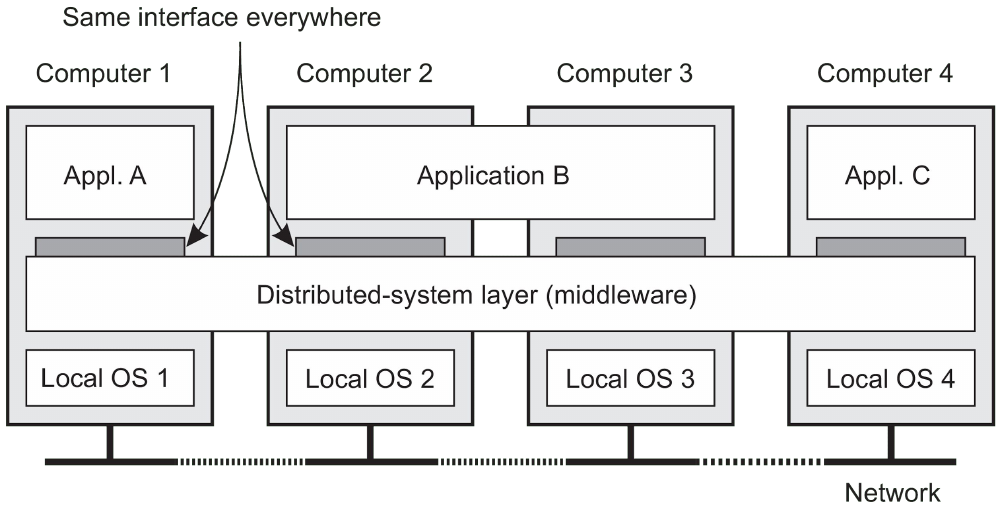
\includegraphics[scale=0.50]{img/middle.png}
			\caption{Livello Middleware}
		\end{figure}
		Il \textbf{middleware} è un insieme di applicazioni e protocolli "\textbf{general purpose}" che risiedono all'interno del livello applicativo. è dunque un livello software che astrae dall'eterogeneità di rete, hardware, sistemi operativi e linguaggi di programmazione, con lo \textbf{scopo di fornire interfacce comuni che assicurino  modelli di comunicazione e di computazione uniformi}.  Questo livello, dunque, costituisce un insieme di protocolli condivisi dalle applicazioni più specifiche al livello soprastante.
		In sintesi, un livello middleware offre servizi alle applicazioni quali:
		\begin{itemize}
			\item Comunicazione;
			\item Meccanismi di sicurezza;
			\item Transazioni
			\item Error-recovery;
			\item Gestione di risorse condivise.
		\end{itemize}
		\textbf{Questi servizi sono indipendenti rispetto alle specifiche applicazioni.} 
		Alcuni esempi:
		\begin{itemize}
			\item Protocolli di autenticazione e autorizzazione (criptografia ssh)
			\item Protocolli di commit. Sono utilizzati per realizzare l'atomicità nelle transazioni. Stabiliscono se in un insieme di processi tutti hanno svolto una particolare operazione o se non è stata svolta affatto.
		\end{itemize}
		Nello specifico vedremo come i \textbf{protocolli di comunicazione middleware supportino servizi di comunicazione ad alto livello} e permettano, per esempio, la chiamata a procedure o oggetti remoti in modo \textbf{trasparente.}
			 
	\subsection{Coordinazione diretta}	
		Un tipi di comunicazione nella quale le componenti partecipanti sono:
		\begin{itemize}
			\item \textbf{Referentially coupled}: durante la comunicazione gli attori utilizzano riferimenti espliciti ai loro interlocutori.
			\item \textbf{Temporally coupled}: entrambe le componenti devono essere in esecuzione (up and running).	
		\end{itemize}
		Il libro propone un'introduzione ai tipi di comunicazione (persist, transient, synchronous, asynchronous).
		
	\subsection{Remote Procedure Call}
		Molti sistemi distribuiti sono basati sullo scambio di messaggi tra processi, tuttavia questo tipo di approccio non permette di nascondere la comunicazione tra le componenti in modo da rendere trasparente il contesto distribuito. \\
		Una soluzione al problema è stata proposta da Nelson e Birrell (1984) introducendo una modalità completamente differente nella gestione della comunicazione nel contesto di un sistema distribuito.
		In breve la proposta è quella di chiamare procedure che sono localizzate su macchine remote:
		\begin{enumerate}
			\item quando A chiama B il processo chiamante in A è sospeso;
			\item l'esecuzione della procedura chiamata ha luogo in B;
			\item A invia i parametri della chiamata a B che a sua volta risponderà con il risultato della chiamata;
			\item \textbf{Nessun passaggio di messaggi è visibile dal punto di vista del programmatore.}
		\end{enumerate}
		La soluzione ha le seguenti problematiche:
		\begin{itemize}
			\item le procedure chiamante e chiamato si trovano su macchine diverse e non condividono lo stesso address space;
			\item la rappresentazione dei parametri e del risultato di ritorno può differire sulle macchine interessate;
			\item Le due macchine potrebbero crashare.
		\end{itemize}
		\begin{figure}[h!]
			\centering
			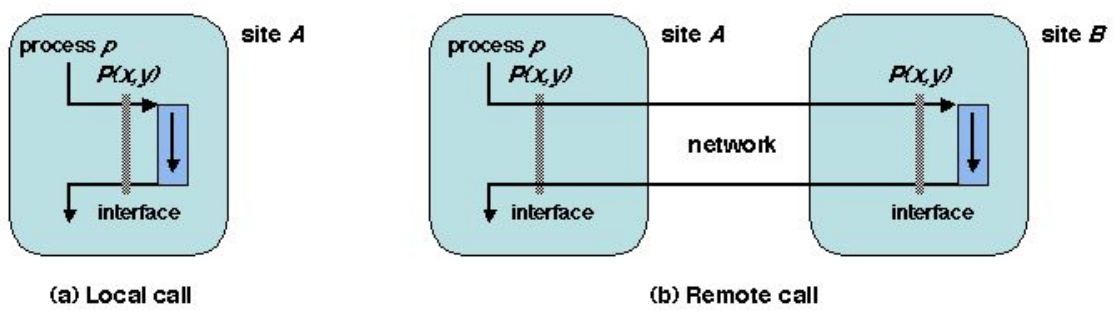
\includegraphics[scale=0.50]{img/proc.png}
			\caption{Chiamata a procedura locale vs remota}
		\end{figure}
		\begin{figure}[h!]
			\centering
			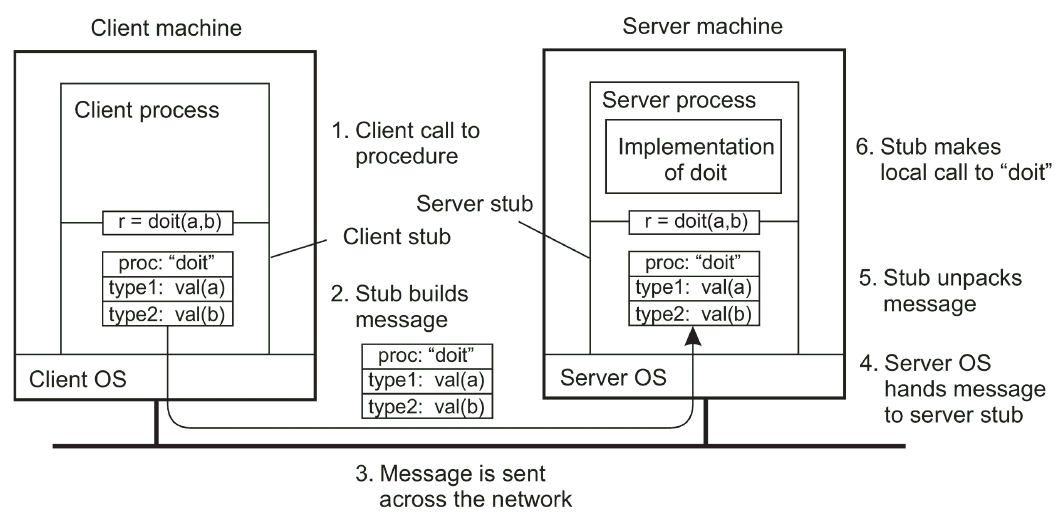
\includegraphics[scale=0.50]{img/how.png}
			\caption{Funzionamento RPC}
		\end{figure}
		Una chiamata a procedura remota deve essere \textbf{trasparente} rispetto al chiamante, per farlo viene creato uno stub locale della funzione che si trova in macchina remota. Lo stub, sia sul server che sul client implementa serializzazione e invio dei parametri e del risultato.  
		Di seguito si elencano i passi necessari ad una chiamata a procedura remota:
		\begin{enumerate}
			\item la procedura del client chiama il proprio stub;
			\item lo stub costruisce il messaggio ed effettua una chiamata al proprio OS;
			\item l'OS del client invia il messaggio all'OS remoto;
			\item l'OS remoto invia il messaggio allo stub del server;
			\item lo stub del server decomprime i parametri e chiama la procedura locale sul server;
			\item si esegue la computazione e si invia i risultati allo stub; 
			\item lo stub del server comprime i risultati e li invia al proprio OS;
			\item si invia il messaggio all'OS del client che lo passa allo stub del client;
			\item lo stub decomprime il risultato della computazione e lo passa al client
		\end{enumerate}
		
		\subsubsection{Passaggio di parametri}
			L'operazione di impacchettare parametri all'interno di un messaggio è chiamata \textbf{marhaling}, il messaggio conterrà i parametri stessi e le informazioni necessarie al destinatario. Il principale problema è il seguente: \textbf{client e server potrebbero adottare diverse rappresentazioni per i dati} (esempio diverse little endian big endian). Nel caso di utilizzo di HTTP come protocollo di trasporto il formato xml può essere utilizzato come formato comune per il passaggio dei parametri.
			\begin{figure}[h!]
				\centering
				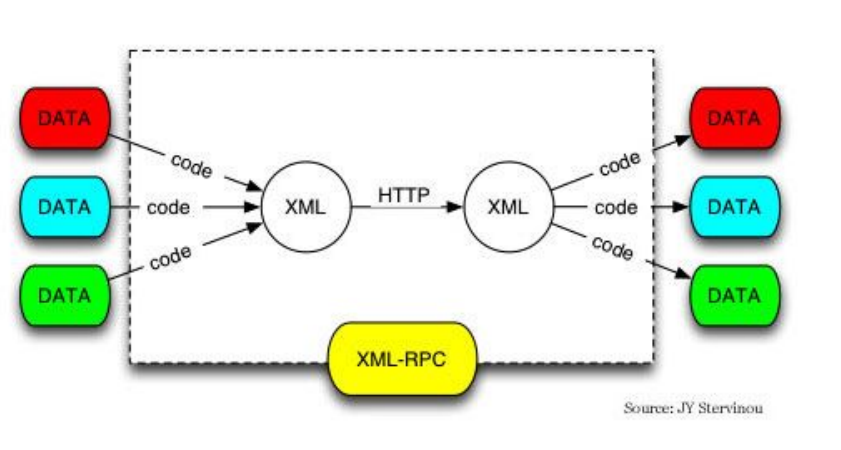
\includegraphics[scale=0.50]{img/xml.png}
				\caption{Xml }
			\end{figure}
		
			\textbf{Un problema} ulteriore risiede nel \textbf{passaggio dei puntatori e riferimenti}. Infatti, questi avranno senso solo se riferiti allo spazio di indirizzi locale del chiamante. Una possibile soluzione è quella di sostituire la \textbf{chiamata per riferimento} con un \textbf{copia/ripristina}. L'idea è quella di effettuare una copia dell'array da passare ed allegarla al messaggio destinato al server. L'array è conservato in un buffer nello stub del server ed inviato nuovamente al client una volta effettuata la chiamata remota (se richiesto). Nonostante i linguaggi offrano supporto automatico al \textbf{(un)marshaling}, quest'ultimo introduce un'\textbf{overhead} nella comunicazione, soprattutto in caso di grosse strutture dati come alberi e grafi.
			
			\begin{figure}[h!]
				\centering
				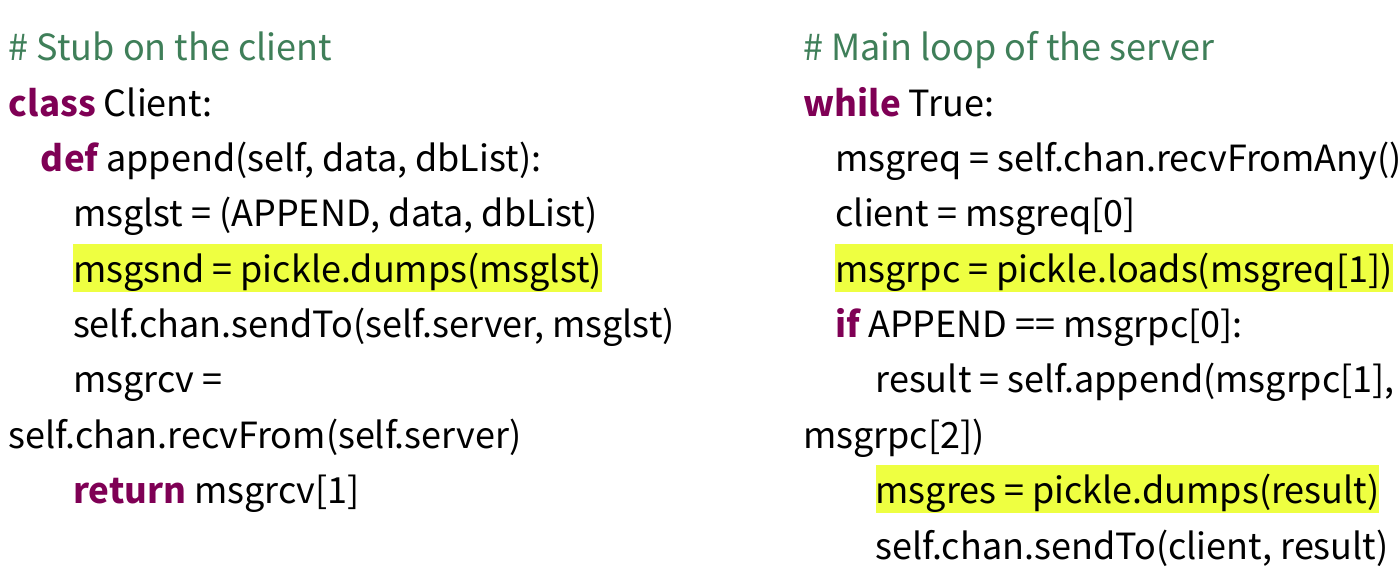
\includegraphics[scale=0.25]{img/rpccode.png}
				\caption{Marshaling in Java  }
			\end{figure}   
		
			Il problema non si presenta qualora i riferimenti siano \textbf{globali}, ovvero quando hanno un significato sia per il server sia per il client. \newline
			In generale, nel contesto di un sistema basato sugli oggetti sono definite due tipologie di oggetti:
			\begin{itemize}
				\item \textbf{Locali}: copiati e trasmessi nella loro interezza;
				\item \textbf{Remoti}: solo lo stub è copiato e trasmesso. 
			\end{itemize}
			In Java oggetti remoti o locali hanno tipi diversi (i remoti implementano l'interfaccia Remote).
			\begin{figure}[h!]
				\centering
				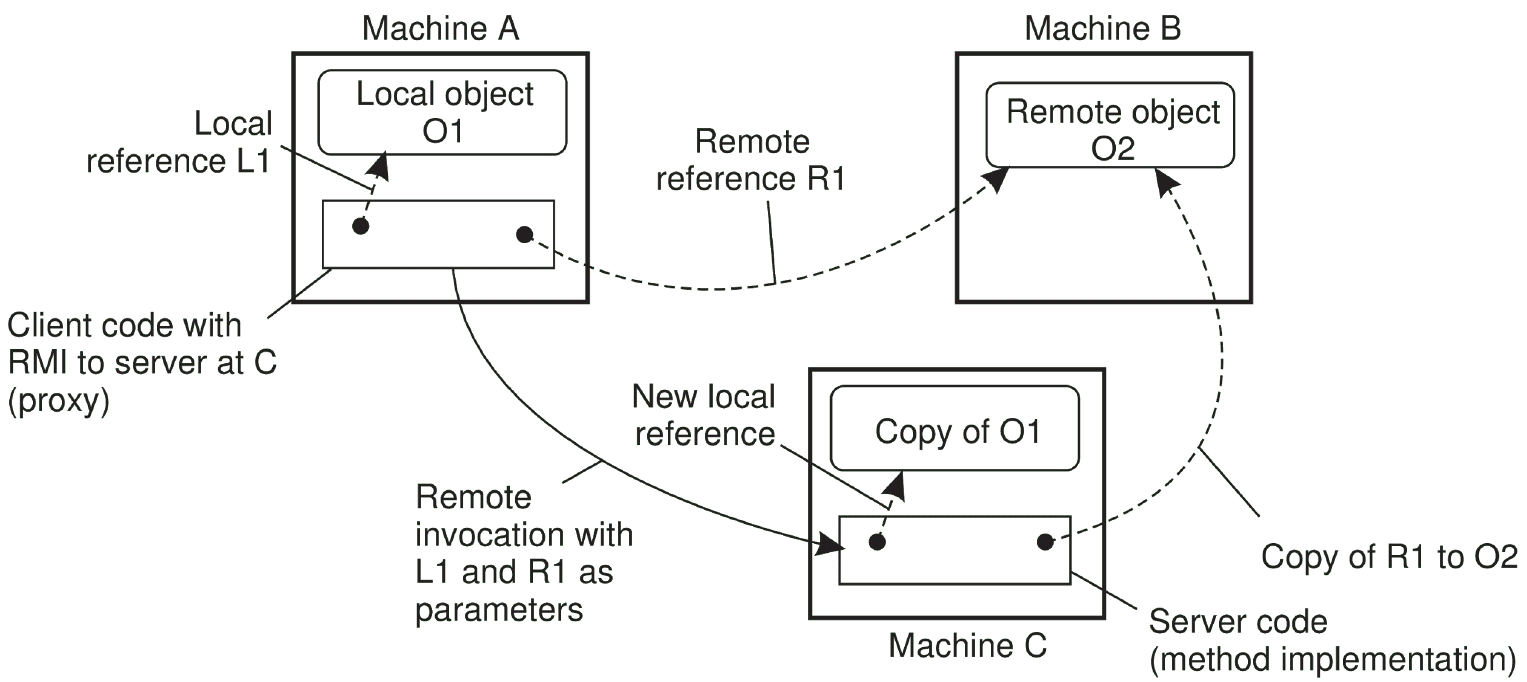
\includegraphics[scale=0.25]{img/remotelocal.png}
				\caption{Oggetti remoti e locali  }
			\end{figure}
		
		\subsubsection{Implementare RPC}
			Ci sono due modi attraverso il quale il meccanismo RPC può essere fornito allo sviluppatore:
			\begin{itemize}
				\item \textbf{Framework o libreria}: il programmatore deve specificare cosa è esportato in remoto fornendo di fatto un'\textbf{interfaccia del servizio}, che contiene tutte le procedure che possono essere chiamate dal client. I framework hanno il pregio di essere \textbf{indipendenti dal linguaggio}. Per questo è norma utilizzare un \textbf{Interface Definition Language (IDL)} che, una volta compilato, genere gli stub per client e server nel linguaggio desiderato. Di contro non abbiamo trasparenza totale per il programmatore che dunque è consapevole di trovarsi nel contesto di una chiamata a procedura remota (deve specificare egli stesso gli oggetti remoti). Alcuni esempi di framework: \textbf{Corba, GRPC, Apache Thrift}.     
				\item \textbf{Costrutti all'interno del linguaggio}: è lo stesso linguaggio a definire i costrutti necessari ad una RPC. In questo caso è il \textbf{compilatore a generare gli stub} per client e server. In questo modo si ottiene \textbf{trasparenza} per il programmatore, tuttavia client e server devono essere \textbf{implementati nello stesso linguaggio} (Es: \textbf{Java RMI}).
			\end{itemize}
		
		\subsubsection{RPC Asincrono}
			\begin{figure}[h!]
				\centering
				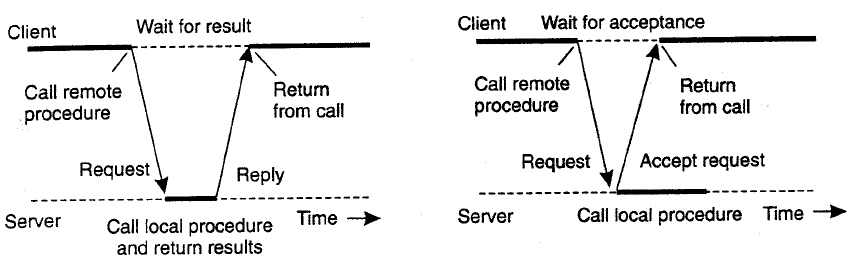
\includegraphics[scale=0.45]{img/async.png}
				\caption{RPC tradizionale e asincrona }
			\end{figure}
			A differenza del paradigma tradizionale nel quale il client attende la risposta del server bloccando la sua esecuzione, il server invia un ACK al client una volta ricevuta la richiesta. L'ACK viene inviato al client per notificare che la sua richiesta sarà processata, nel frattempo il client può eseguire ulteriori operazioni evitando di sospendere la sua esecuzione. Il Server utilizza una funzione detta di \textbf{Callback} per consegnare il risultato al Client.
			\begin{figure}[h!]
				\centering
				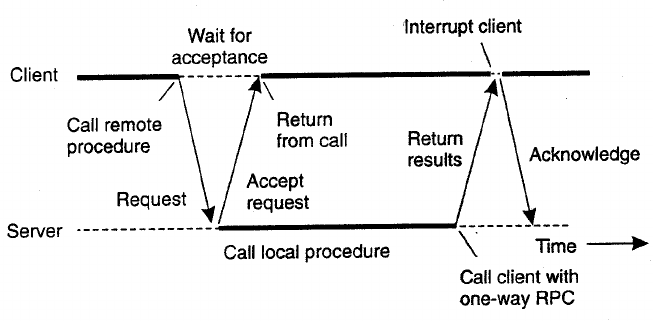
\includegraphics[scale=0.40]{img/callback.png}
				\caption{Callback }
			\end{figure}
			L'asincronicità della comunicazione permette l'implementazione di un protocollo \textbf{Multicast RPC} inviando richieste in parallelo a server diversi che dunque processano indipendentemente l'uno dall'altro. Si può definire questo protocollo nell'ottica di accettare il risultato più veloce scartando dunque gli altri, oppure per la realizzazione di una computazione distribuita, combinando i risultati ricevuti.
			
		\subsubsection{Binding}
			In applicazioni reali abbiamo bisogno di una fase preliminare chiamata \textbf{binding} che permette al client di avere un riferimento al server. Necessario per il client risulta l'utilizzo di un \textbf{registro} al cui interno sono salvate coppie (nome, indirizzo) di uno o più server. Si utilizza tale riferimento per la comunicazione.
			\begin{figure}[h!]
				\centering
				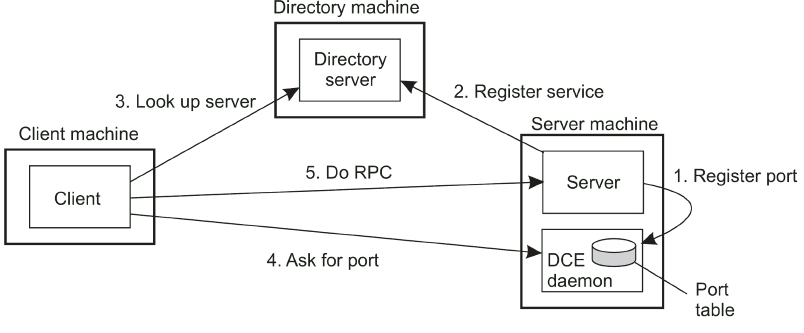
\includegraphics[scale=0.45]{img/bind.png}
				\caption{Binding }
			\end{figure}
		
	\subsection{Message Oriented Middleware}
		Questo modello di comunicazione prevede lo scambio di messaggi tra le entità partecipant. Grazie allo scambio di messaggi possiamo definire un modello nel quale, mittente e destinatario \textbf{non devono essere attivi durante lo scambio dei messaggi}. Questo è possibile grazie al Middleware che mette a disposizione buffer temporanei per i messaggi scambiati. Ogni applicazione ha a disposizione una coda locale che contiene i messaggi inviati e ricevuti e che può eventualmente essere condivisa tra più applicativi.
		\begin{figure}[h!]
			\centering
			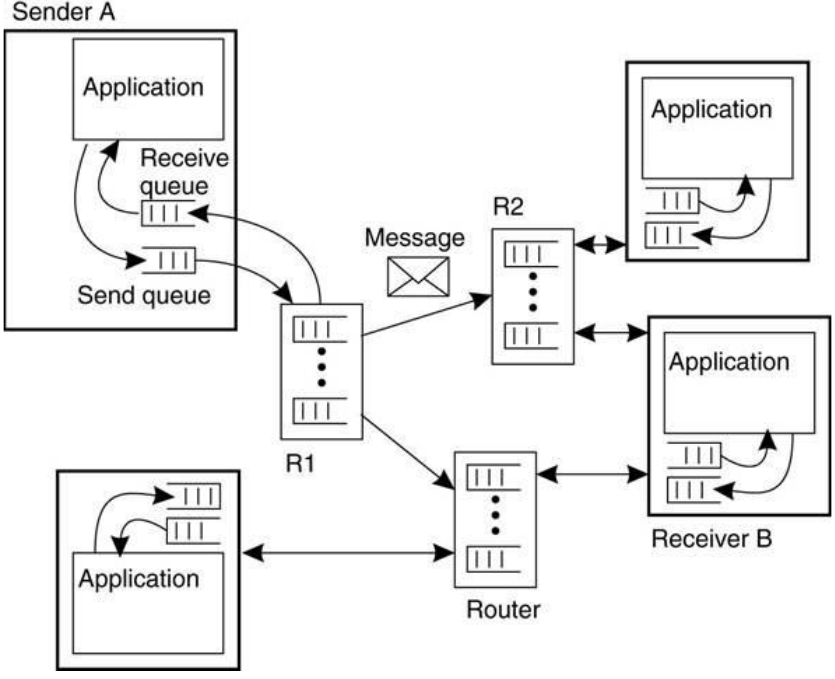
\includegraphics[scale=0.30]{img/queque.png}
			\caption{Code }
		\end{figure} 
		Il modello di comunicazione definito ha le seguenti proprietà:
		\begin{itemize}
			\item La comunicazione avviene semplicemente inserendo e rimuovendo messaggi dalla coda, un messaggio ovviamente rimane nella coda fino a che non è esplicitamente rimosso;
			\item La comunicazione è \textbf{loosely coupled}, cioò significa che il ricevente non deve essere necessariamente in esecuzione.   
		\end{itemize}
		Di seguito sono elencate le primitive concettuali che un message oriented middleware deve esporre:
		\begin{itemize}
			\item \textbf{Put}: inserisce un messaggio nella coda;
			\item \textbf{Get}: rimuove il primo messaggio dalla coda (blocking);
			\item \textbf{Poll}: rimuove il primo messaggio dalla coda (non-blocking);
			\item \textbf{Notify}: informa che un messaggio è arrivato nella coda.	
		\end{itemize}
		\newpage
		
		\subsubsection{Queue Manager}
			Il queue manager gestisce i messaggi inviati o ricevuti da un'applicazione nella sua coda (ad ogni applicazione è associata una coda e un relativo manager). Può essere implementato come una libreria collegata all'applicazione o come un \textbf{processo separato}. \textit{Nel secondo caso il sistema supporterà la comunicazione asincrona persistente}.
			\begin{figure}[h!]
				\centering
				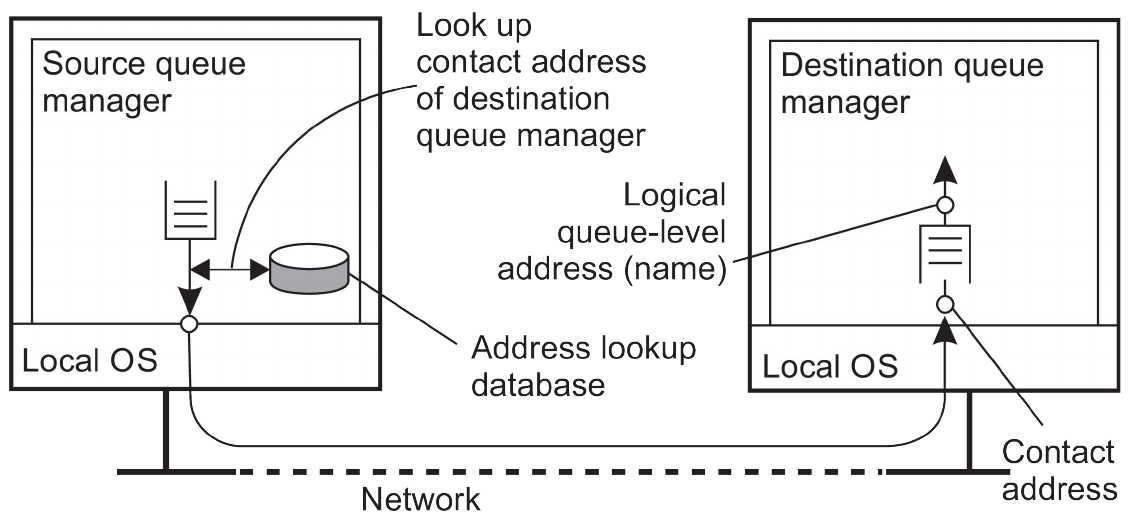
\includegraphics[scale=0.30]{img/mana.png}
				\caption{Queue Manager }
			\end{figure}
			In definitiva questi processi operano come \textbf{router} o \textbf{relay} inoltrando i messaggi ricevuti ad altri queue manager. In questo modo il sistema di quequing può costituire \textbf{un livello applicazione a se stante (Overlay network )} (un'astrazione), basato su una rete di computer esistente.
			\begin{figure}[h!]
				\centering
				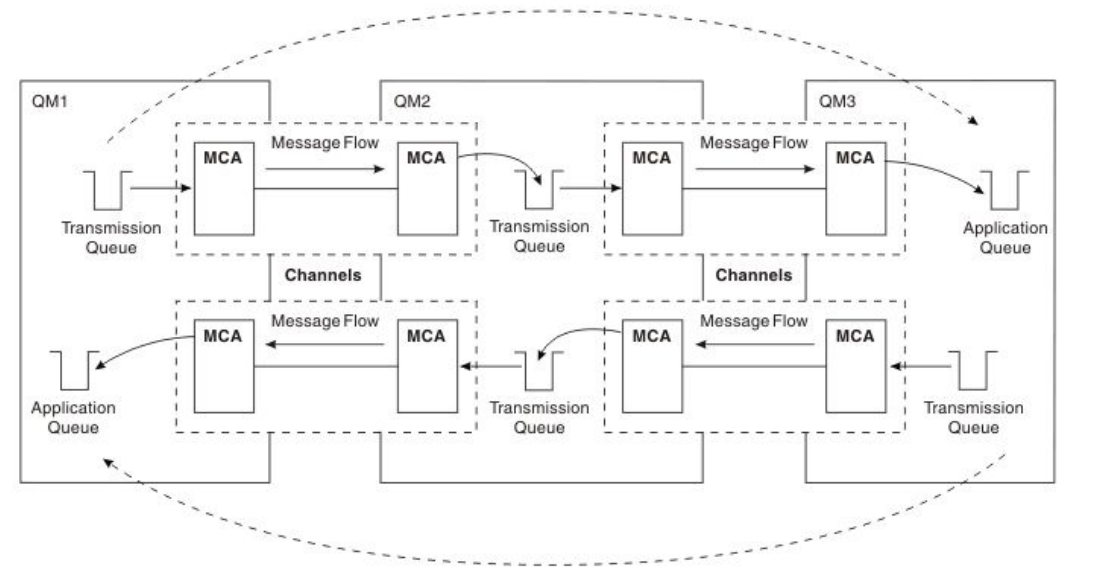
\includegraphics[scale=0.40]{img/overlay.png}
				\caption{Overlay network }
			\end{figure}
			Questa overlay network deve essere collegata e per farlo ogni entità deve essere a conoscenza degli indirizzi fisici associati ai nomi delle macchine partecipanti la rete e quindi delle loro rispettive code. Questo approccio \textbf{non risulta scalabile} e nel contesto di reti di grosse dimensioni porta ad evidenti \textbf{problemi gestionali}. Possiamo migliorare il modello di comunicazione delegando ai router la responsabilità di tenere traccia della topologia di rete e di aggiornare i binding (nome, indirizzo), mentre le altre entità partecipanti possiedono dei riferimenti statici al/ai router più vicino.
			
		\subsubsection{Eterogeneità: Message Brokers}
			I sistemi distribuiti possono essere eterogenei rispetto ai linguaggi utilizzati per realizzare le singole entità partecipanti. In questi casi è difficile definire un protocollo condiviso poichè è assente alla base un'accordo sul formato dei dati messaggi scambiati.\\
			Un \textbf{Message Broker} si comporta come un getway: si occupa di convertire i messaggi ricevuti in un formato consono a quello del ricevente. Nella pratica un message broker usa un repository di regole e programmi che permettono la conversione di un messaggio T1 in uno T2.
			Esempi di message brokers: 
			
	\subsection{Java RMI}
		Java RMI (\textbf{Remote Method Invocation}) è un framework che permette di implementare il modello RPC nel constesto di un sistema distribuito.
		\begin{figure}[h!]
			\centering
			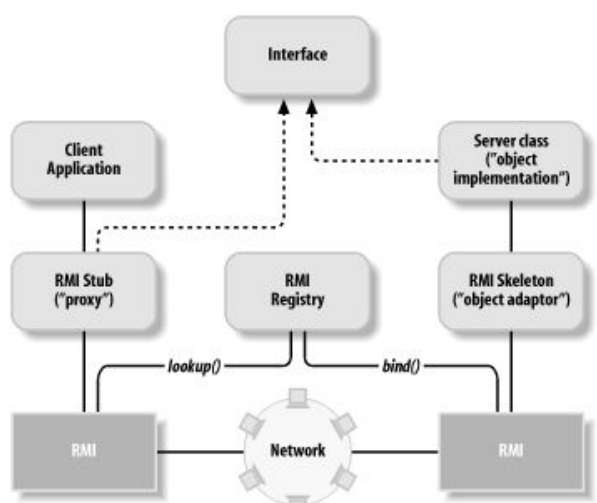
\includegraphics[scale=0.40]{img/rmi.png}
			\caption{Architettura di RMI}
		\end{figure}
		Il modello presenta 4 entità principali:
		\begin{itemize}
			\item \textbf{Interfaccia}: utilizzata per definire la risorsa remota;
			\item \textbf{Server}: implementa la risorsa remota (che sarà richiesta dal client);
			\item \textbf{Client}: richiede al server la risorsa remota.
			\item \textbf{Registro}: si occupa di gestire l'accesso alla risorsa remota.
		\end{itemize}
		Il \textbf{Registro}: è un servizio di \textbf{naming} che mappa i nomi simbolici degli oggetti remoti al loro stub. Il Server può registrare un oggetto remoto nel registro scrivendone il nome e l'indirizzo al quale è reperibile. Il client cerca l'oggetto remoto all'interno del registro.\\
		L'\textbf{interfaccia} specifica un contratto, ovvero le firme dei metodi che si possono invocare sull'oggetto remoto e che dunque ne regolano le modalità di utilizzo. \textbf{Per ogni oggetto} che vogliamo rendere accessibile attraverso la rete dobbiamo definire un'interfaccia che estenda l'interfaccia remota \textit{\textbf{java.rmi.remote}}. Le interfacce così definite dal server devono essere note anche al client in modo tale che egli possa operare sugli oggetti ricevuti dal server senza incorrere in errori di tipo. L'interfaccia remota serve solo ad indicare la possibilità di reperire gli oggetti che estendono tale interfaccia in remoto.\\
		Vediamo quali sono i passi per implementare un \textbf{RMI server}:
		\begin{enumerate}
			\item Implementare la classe remota definendo costruttore e metodi remoti (estendiamo la classe \textit{\textbf{java.rmi.server.UnicastRemoteObject }} e ne chiamiamo il costruttore per esportare l'oggetto);
			\item Creare un'istanza dell'oggetto remoto;
			\item Registrare tale oggetto remoto all'interno del registro. Per fare questo dobbiamo scegliere un identificativo unico (una stringa) per l'oggetto, che deve essere noto anche al client. Una volta ottenuto un riferimento al registry creiamo un binding tra quel nome e l'istanza dell'oggetto relativa. La classe \textit{\textbf{LocateRegistry}} permette di ottenere il riferimento al registro remoto o di crearne uno in ascolto sulla porta desiderata sullo stesso host del server (\textbf{\textit{createRegistry(int port), getRegistry(String host, int port )}}). 
		\end{enumerate}
		Per quanto riguarda il client i passi per l'implementazione sono i seguenti:
		\begin{enumerate}
			\item Localizzare il registro (stessi metodi della classe \textbf{LocateRegistry} indicati per il server);
			\item Utilizzare un nome simbolico per cercare l'oggetto remoto all'interno del registro;
			\item utilizzare l'oggetto remoto chiamandone i metodi. 
		\end{enumerate}
		Possiamo utilizzare RMI per implementare una comunicazione \textbf{sincrona} (il client aspetta fino al termine dell'invocazione remota). Possiamo ottenere una comunicazione \textbf{asincrona} utilizzando le \textbf{callback} il client invoca un oggetto remoto e passa la callback al server (un altro oggetto remoto).
		
	\subsection{gRPC}
		gRPC è un framework open source per l'implementazione del modello RPC:
		\begin{itemize}
			\item Si basa su i meccanismi di streaming messi a disposizione da \textbf{ HTTP/2};
			\item \textbf{Supporta molti linguaggi} grazie all'utilizzo di un \textbf{IDL} (Interface Definition Language).
			\item Si appoggia a \textbf{Protocol Buffer} che è un meccanismo per la serializzazione di strutture dati basato su un particolare formato binario che rendono i payload leggeri e veloci da trasmettere. Mette a disposizione un linguaggio proprio utilizzabile per definire interfacce indipendenti dal linguaggio.
		\end{itemize}
		I servizi messi a disposizione sono 4:
		\begin{itemize}
			\item \textbf{Unary RPCs}: Implementa uno scambio di messaggi \textbf{sincrono}.
			\item \textbf{Server streaming RPCs}: Un client invia richieste al server e riceve uno stream di messaggi (il client legge dallo stream fino a che non ci sono piu messaggi).
			\item \textbf{Client streaming RPCs}: Il client scrive una sequenza di messaggi e li manda al server utilizzando uno stream.
			\item \textbf{Bidirection streaming RPCs}: Entrambi i lati della comunicazione utilizzano uno stream in lettura/scrittura per inviare e ricevere messaggi.  
		\end{itemize}
		Il Workflow di gRPC è il seguente:
		\begin{itemize}
			\item \textbf{Definire un'interfaccia} utilizzando il Protocol Buffer Language ed il suo IDL (file di testo in formato \textbf{.proto});
			\item \textbf{Compilare} l'interfaccia per ottenere gli stub per client e server e le classi necessarrie alla serializzazione (si utilizza il comando \textbf{protoc}).
			\item \textbf{Integrare} gli stub con codice ad-hoc.
		\end{itemize}
		\begin{figure}[h!]
			\centering
			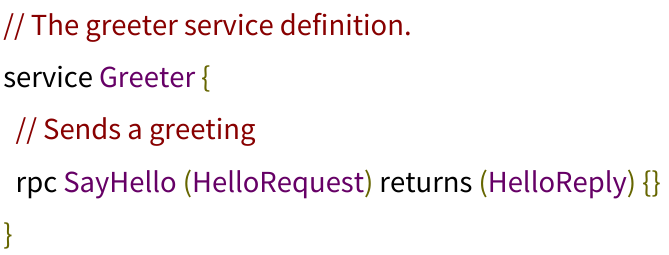
\includegraphics[scale=0.30]{img/idl.png}
			\caption{Definizione di un interfaccia con gRPC IDL}
		\end{figure}
	
		FINIRE SU SLIDE 
		
\section{Basic distributed algorithms}
	\subsection{Contesto}
		Il \textbf{contesto} nel quale operiamo è chiamato \textbf{ambiente distribuito}. Consiste in una collezione finita $\epsilon$ di \textbf{entità} che comunicano attraverso \textbf{messaggi} con lo scopo di raggiungere un \textbf{obiettivo comune}. Vediamo quali sono le componenti principali del modello:
		\begin{itemize}
			\item \textbf{Entità}: è l'unità computazionale di un ambiente distribuito, può essere vista come un processo, un agente, uno switch ecc. Ogni entità è equipaggiata con una memoria privata e non condivisa. La memoria è composta da un insieme di registri, tra i quali spiccano lo \textbf{status register}, che può assumere i valori di \textit{idle, Processing, Waiting}, e l'\textbf{input value register}. Inoltre è possibile settare un \textbf{alarm clock} locale che può essere resettato all'occorrenza.
			\item \textbf{Eventi esterni}: Il comportamento di un'entità è reattivo ed innescato da stimoli esterni. Questi possono essere:
			\begin{itemize}
				\item L'arrivo di un messaggio;
				\item Lo scadere dell'alarm clock;
				\item Impulsi spontanei.
			\end{itemize}
			L'ultimo è l'unico stimolo originato da forze che sono esterne al sistema (come esempio si riporta la richiesta ad un bancomat da parte dell'utente nel sistema ATM server- ATM client)
			\item \textbf{Azioni}: un'entità può svolgere le seguenti \textbf{operazioni}:
		\begin{itemize}
			\item Operazioni sulla memoria locale;
			\item Trasmissione dei messaggi;
			\item (re)set dell'alarm clock;
			\item Cambiare il valore del registro di stato.
		\end{itemize}
			Le azioni sono \textbf{atomiche} (non possono essere interrotte) e \textbf{finite} (devono terminare in tempo finito). L'azione speciale \textbf{nil} permette ad un'entità di non reagire ad uno specifico evento.
			\item \textbf{Comportamenti delle entità}: l'insieme $B(x)$ è una funzione $Statox Evento \rightarrow Azioni$ ovvero una funzione che ad una coppia stato-evento associa un comportamento (può definire un insieme di comportamenti \textbf{deterministico} o \textbf{non deterministico}). Un sistema è detto \textbf{simmetrico} se tutte le entità hanno lo stesso comportamento ($B(x) = B(y) \forall x,y \in E$). Tutti i sistemi possono essere resi simmetrici.
			\textbf{Comunicazioni:} guarda figure.
		\end{itemize}
		\begin{figure}[h!]
			\centering
			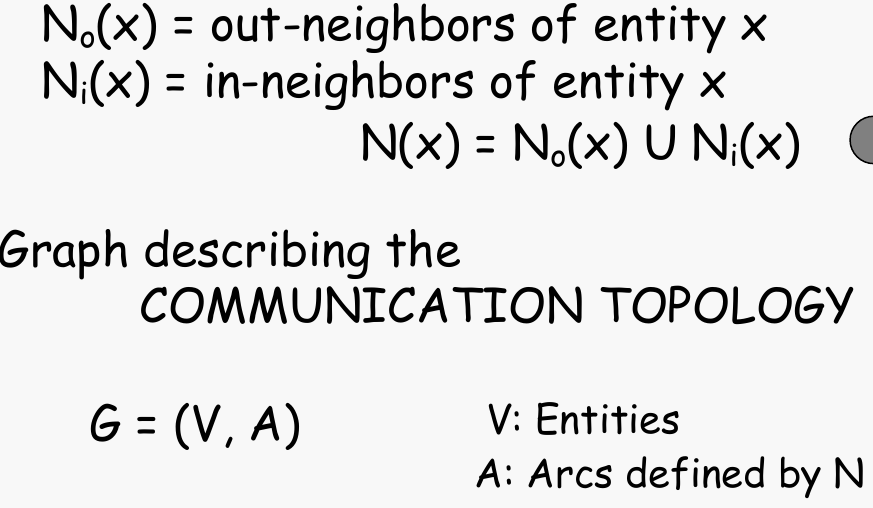
\includegraphics[scale=0.30]{img/comun.png}
			\caption{Come rappresentare la topologia di rete}
		\end{figure}
		\begin{figure}[h!]
			\centering
			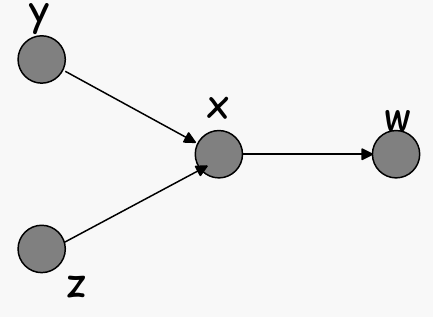
\includegraphics[scale=0.30]{img/graph.png}
			\caption{Topologia}
		\end{figure}
	
		\subsubsection{Assiomi}
			\begin{itemize}
				\item \textbf{Delay trasmissione messaggi}: in assenza di \textbf{fallimenti} un messaggio inviato da x ad un suon vicino y arriva in un tempo finito.
				\item \textbf{Orientamento Locale}: ogni entità può distinguere i suoi \textbf{out-neighbors} ( si utilizzano delle etichette sugli archi). Nella pratica un'entità sa da quale porta il messaggio gli è stato recapitato.
			\end{itemize}
			\begin{figure}[h!]
				\centering
				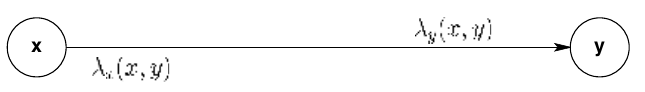
\includegraphics[scale=0.40]{img/lab.png}
				\caption{Labels}
			\end{figure}
		
		\subsubsection{Restrizioni}
			Si possono definire ulteriori proprietà o capacità in relazione ai compiti e agli obiettivi che il sistema distribuito si prepone di raggiungere. Tuttavia queste proprietà aggiuntive  limitano l'applicabilità reale del protocollo e dunque nella pratica rappresentano delle \textbf{restrizioni}. Vediamone alcune:
			\begin{itemize}
				\item \textbf{Ordine dei messaggi:} in assena di fallimenti, messaggi trasmessi nello stesso link arrivano nell'ordine d'invio.
				\item \textbf{Link bidirezionali}: $\forall x$ $N_{i}(x)=N_{o}(x)$ e $\forall y$ $\lambda_{x}(x,y) = \lambda_{x}(y,x	)$ 
				\item \textbf{Fault detection}:
				\begin{itemize}
					\item \textbf{Edge Failure Detection}: un'entità può individuare il fallimento di uno dei suoi link;
					\item \textbf{Entity Failure Detection}: un'entità può rilevare il fallimento di uno dei suoi vicini 	
				\end{itemize} 
				\item \textbf{Reliability restrinction}: 
				\begin{itemize}
					\item \textbf{Guaranteed delivery}: ogni messaggio inviato viene recapitato al mittente non corrotto;
					\item \textbf{Partial reliability}: garantisce l'assenza di fallimenti in futuro;
					\item \textbf{Total reliabilit}: non ci sono stati fallimenti e non ce ne saranno.
				\end{itemize} 
				\item \textbf{Strongly connected}: il grafo g che rappresenta la topologia è fortemente connesso.
				\item \textbf{Knowledge restrinction}
				\begin{itemize}
					\item conoscenza del numero di nodi;
					\item conoscenza del numero di link;
					\item conoscenza del diametro.
				\end{itemize}
			\end{itemize}
		
	\subsubsection{Tempo ed Eventi}
		Un evento esterno genera un'azione che dipende dallo stato dell'entità in questione. Un'azione può a sua volta generare un evento (per esempio l'operazione send genera un evento receiving). Un'ulteriore considerazione riguarda la possibilità che eventi generati in questo modo possano non occorrere nel caso in cui vi sia un fallimento del link di comunicazione. Ovviamente questi eventi se occorrono occorrono dopo del tempo (alla ricezione del messaggio per esempio). Eventi come \textbf{receiving} hanno un \textbf{delay non predicibile}. Un'esecuzione è descritta completamente dalla sequenza di eventi che è occorsa. Delay diversi porteranno ad esecuzioni differenti e dunque a risultati possibilmente diversi. Per convenzione tutti gli eventi spontanei sono generati al tempo $t=0$ prima che l'esecuzione abbia inizio.\\
		Definito $\alpha(x,t)$ lo stato del nodo x al tempo t, è importante evidenziare che:
		\begin{itemize}
			\item se un evento avviene in due esecuzioni diverse e gli stati $\alpha 1$ e $\alpha 2$ sono uguali, allora \textbf{il nuovo stato interno sarà lo stesso in entrambe le esecuzioni}.
			\item se un evento avviene al tempo t nei nodi x e y ed i loro stati $\alpha(x)$ e $\alpha(y)$ sono uguali, allora i nuovi stati di x e y saranno lo stesso stato.
		\end{itemize}
		
		
		\begin{figure}[h!]
			\centering
			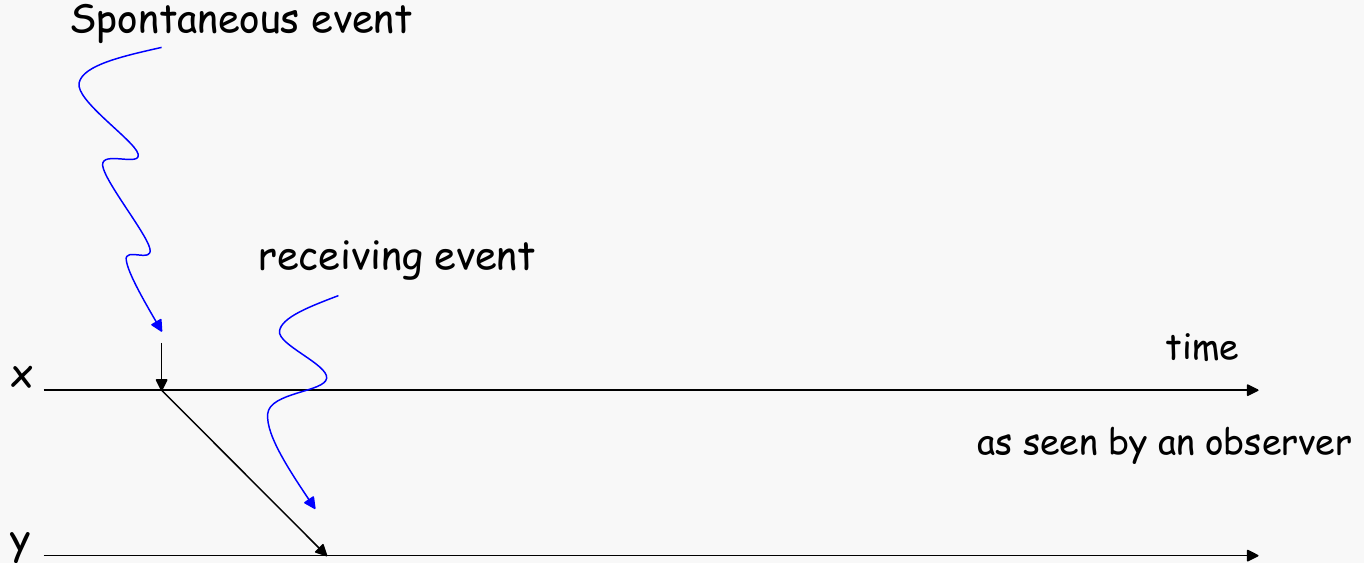
\includegraphics[scale=0.25]{img/event.png}
			\caption{Stato x Evento}
		\end{figure}
	
	\subsubsection{Livelli di Conoscenza}
		\begin{itemize}
			\item \textbf{Local knowledge}: $p \in LK_t[x]$ dove p è il contenuto della memoria locale di un'entità e tutte le informazioni derivabili da essa.
			\item \textbf{Implicit knowledge}: $p \in IK_t[W]\_ iff \exists x \in W$ $(p \in LK_t[x])$
			\item \textbf{Explicit knowledge}: $p \in EK_t[W]\_ iff \forall x \in W$ $(p \in LK_t[x])$
		\end{itemize}
		I \textbf{tipi di conoscenza} includono quelle \textbf{topologiche}, \textbf{metriche} (numero di nodi, diametro, eccentricità), \textbf{senso della direzione} (informazioni sui link, informazioni sulle label). Importante sottolineare come \textbf{al crescere delle conoscenze l'algoritmo diventi meno portatile}. Gli algoritmi generici non utilizzano nessuna conoscenza.     
	
	\subsection{Broadcast}
		Considerato un sistema distribuito nel quale solo il nodo x sia a conoscenza di una qualche informazione importante, il \textbf{problema del broadcast} consiste nel propagare questa informazione a tutti gli altri nodi. Una soluzione del problema deve essere valida a prescindere dal nodo \textbf{iniziatore}.
		
		\subsubsection{Flooding}
			\textbf{Assunzioni}: (\textbf{{BL, CN, TR}}) Bidirectional link, Connectivity (ogni entità è capace di raggiungere l'altra), Total reliability. + (\textbf{UI+}).\\
			Una soluzione al problema del broadcast è data dall'algoritmo \textbf{flooding}. L'idea è molto semplice: se un nodo è a conoscenza di qualcosa invia l'informazione ai suoi vicini. L'algoritmo è riportato in figura nella variante per la quale il mittente viene escluso dalla lista dei nodi ai quali inoltrare l'informazione ricevuta.
			\begin{figure}[h!]
				\centering
				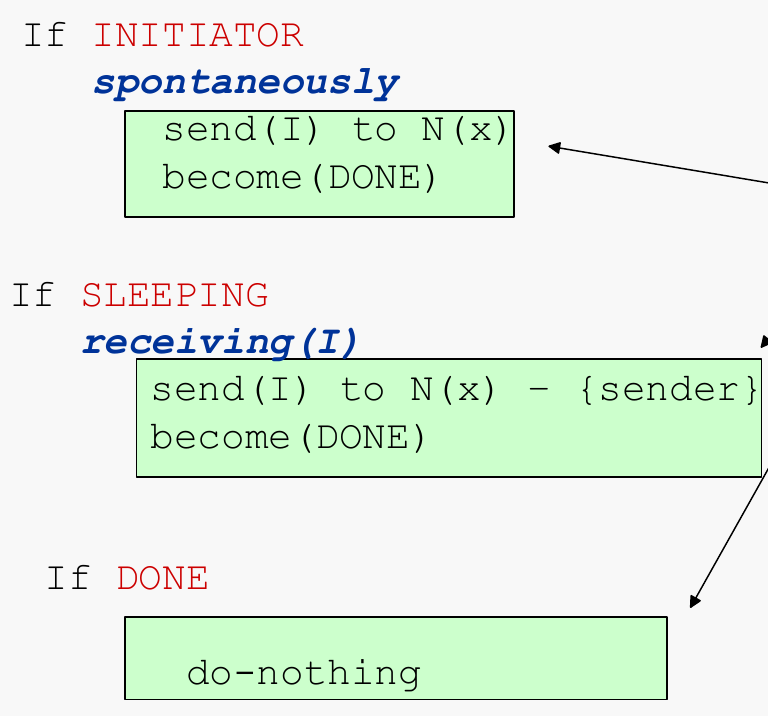
\includegraphics[scale=0.4]{img/flood.png}
				\caption{Algoritmo Flooding}
			\end{figure}
		L'algoritmo gode della proprità di \textbf{Termination}: l'algoritmo termina in tempo finito (local termination quando lo stato è \textit{done}). Garantita dal fatto che il grafo è connesso e che vale la proprietà di total reliability. Il caso peggiore si presenta quando il \textbf{grafo è completo}.\\
		Per quanto riguarda la \textbf{complessità dei messaggi}: vengono scambiati 2 messaggi per ogni link $$\sum_{x}^{}N(x)=2m \rightarrow 2m = O(m) $$ nello specifico:
		$$|N(s)|+\sum_{x\neq s}^{}(N(x)-1)=\sum_{x}^{}(N(x)-\sum_{x}^{}1) = 2m-(n-1)$$
		Per quanto riguarda la complessità in tempo abbiamo:
		$$r(s)=Max_x(d(x,s))=eccentricity \leq Diameter(G) \leq n-1$$
		con:
		$$Diameter(G)=Max_x(r(x))  $$
		
		
	\subsection{Flooding in reti con caratteristiche particolari}
		Un algoritmo che implementi il broadcast in un sistema distribuito varia la sua efficienza in base alla topologia di rete. Vediamo alcuni casi:
		\subsubsection{Broadcast in un Hypercube}
			Per $k=1$ un hypercube è un grafo che presenta due nodi collegati da un link.
			Un Hypercube $H_k$ di dimensione $k>1$ è ottenuto prendendo due hypercube di dimensione $k-1-H^{1}_k-1$ e collegando i nodi con nome uguale con un link etichettato. I nuovi nomi dei nodi sono ottenuti aggiungendo il prefisso 1 o il prefisso 0 ai nomi precedenti. Le label dei link sono ottenute contando i bit di differenza tra il nome dei due nodi collegati. Le etichette sono simmetriche rispetto ai nodi connessi dal link\\
			\begin{figure}[h!]
				\centering
				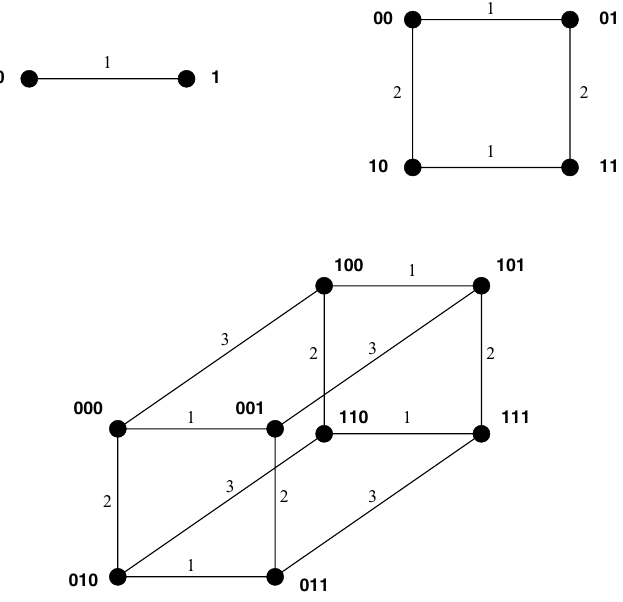
\includegraphics[scale=0.35]{img/hyper.png}
				\caption{Hypercube}
			\end{figure}
			\begin{figure}[h!]
				\centering
				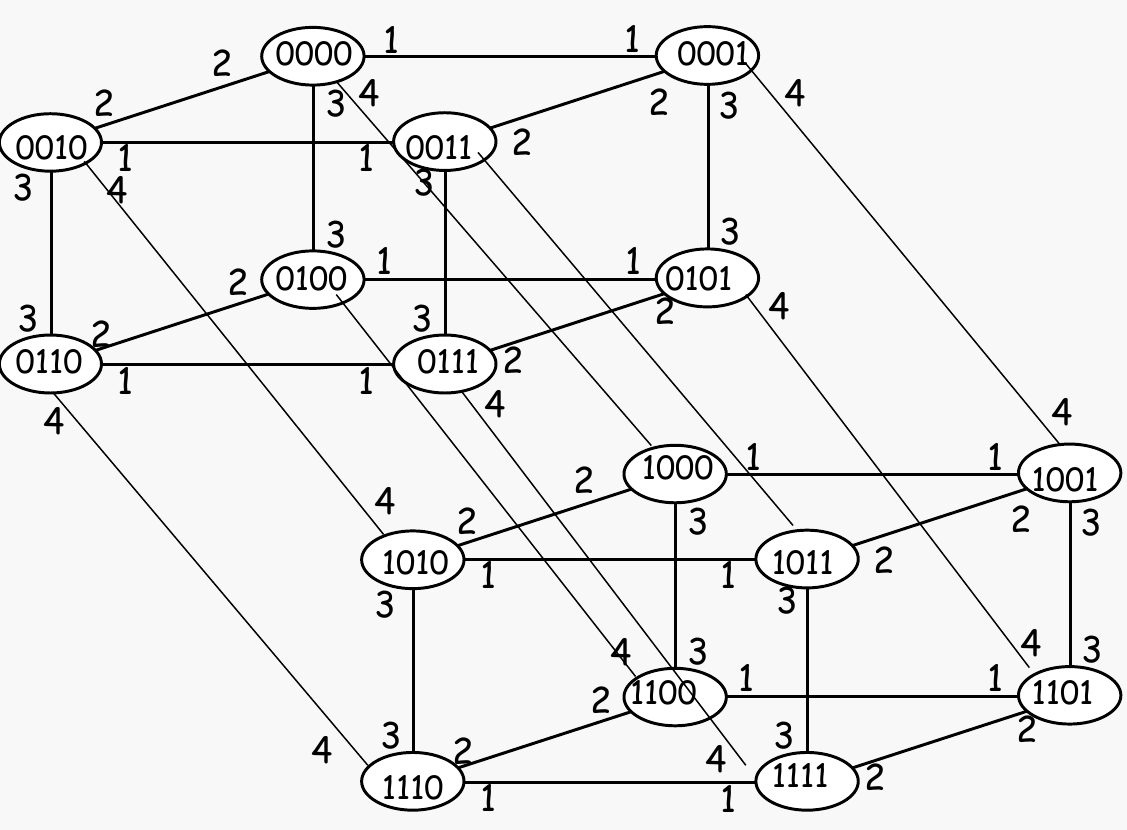
\includegraphics[scale=0.20]{img/hyper2.png}
				\caption{Costruzione hypercube}
			\end{figure}
			\textbf{\textit{Ricordiamo che i nomi dei nodi sono utilizzati solo a scopo descrittivo e non sono conosciuti dalle entità. Al contrario in nomi delle etichette sono noti alle entità per l'assioma di local orientation}.}\\
			Vediamo la \textbf{complessità} del flooding per questa particolare topologia. Un hypercube di dimensione $k$ ha $n=2^{k}$ \textbf{nodi}. Pertanto il \textbf{numero di link è}:
			$$m=nk/2= O(nlog(n)) $$ il costo del flooding è pertanto:
			$$2m-(n-1) = nlog(n)-(n-1)=(nlog(n)/2) +1=O(nlog(n))$$
			Possiamo utilizzare le proprietà topologiche dell'hypercube per ottenere un broadcast ancora più efficiente:
			\begin{enumerate}
				\item L'iniziatore invia il messaggio a tutti i suoi vicini;
				\item Un nodo che riceve un mesaggio dal link $l$, lo invia solo ai link con etichetta $l^{1}<l$ 
			\end{enumerate}
			Con questa modifica il flooding costerà soltanto (n-1) (messaggi).\\
			La \textbf{correttezza} dell'algoritmo è data dal seguente lemma: \textit{per ogni paio di nodi x,y esiste un path unico di etichette decrescenti}.
			\begin{figure}[h!]
				\centering
				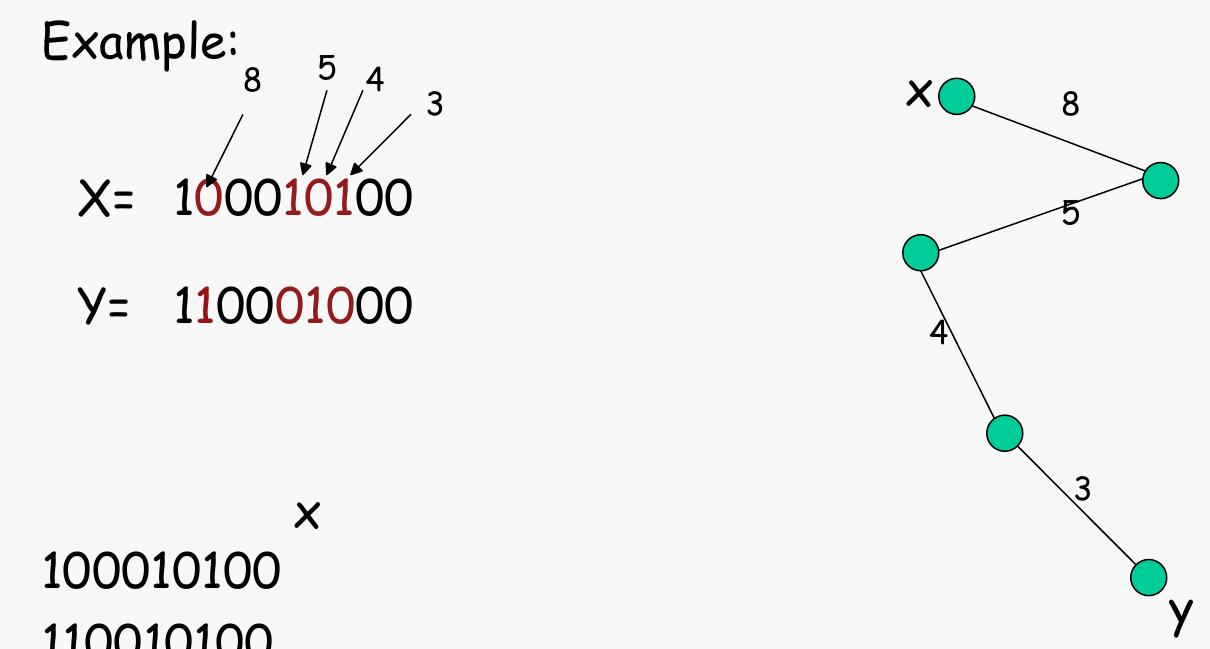
\includegraphics[scale=0.20]{img/hyper3.png}
				\caption{Lemma}
			\end{figure}
			Il risultato è che il messaggio crea uno \textbf{spanning tree} e ogni nodo è raggiunto da tale messaggio. La complessità risulta essere quella ottimale (n-1) perchè le entità ricevono l'informazione solo una volta. La complessità ideale in tempo è k poichè l'eccentricità di ogni nodo è k.
		\subsubsection{Broadcast in un grafo completo}
			Notiamo che nel caso di un grafo completo il flooding ha complessità 
			$$2m-(n-1)=O(n^{2}) $$ con complessità per i messaggi di:
			$$(n-1) $$
		\subsubsection{Lower bound}
			Torniamo al caso generale del broadcast e cerchiamo una limitazione inferiore per la sua complessità.\\ \textbf{Teorema}:\\
			\textit{Ogni algoritmo di broadcast richiede, nel caso pessimo, O(m) messaggi}.\\
			La prova avviene per contraddizione: sia A un algoritmo che esegue broadcast in meno di m(G) messaggi. In questo caso abbiamo almeno un link in G dove nessun messaggio inviato.
			
			VEDERE DIMOSTRAZIONE
			
	\subsection{Spanning tree construction}
		Per ottimizzare il costo di un algoritmo distribuito può essere una buona soluzione quella di ottenere una topologia di rete con particolari caratteristiche. è questo il caso degli \textbf{spanning tree}.\\
		Nella teoria dei grafi uno spanning tree T di un grafo \textbf{aciclico} è un suo sottografo che include tutti i vertici di G con il numero minore possibile di archi. Lo spanning tree per un grafo G \textbf{non è unico}.
		\subsubsection{Protocollo Shout}
			Grazie all'assioma di \textbf{local orientation} un'entità è consapevole solo delle etichette delle porte con le quali comunica con i suoi vicini. Inoltre sappiamo che i messaggi inviati ad un vicino sono prima o poi ricevuti dal destinatario (grazie all'assioma di \textbf{finite comunication delay} e la restrizione di \textbf{total reliability}). In questa configurazione iniziale un'entità ha bisogno di conoscere \textit{solo chi tra i suoi vicini è anche suo vicino nello spanning tree}. Vediamo la strategia utilizzata:
			\begin{enumerate}
				\item L'iniziatore \textbf{s} invia un messaggio ai suoi vicini \textbf{"\textit{sei tu il mio vicino?}"};
				\item un'entità $x\neq s$ risponde "\textit{\textbf{yes}"} solo la prima volta ed in questa occasione pone a tutti i suoi vicini la stessa domanda, altrimenti risponde "\textbf{\textit{no}}".
				\item Ogni entità termina quando ha ricevuto una risposta da tutti i vicini. 
			\end{enumerate}
			\begin{figure}[h!]
				\centering
				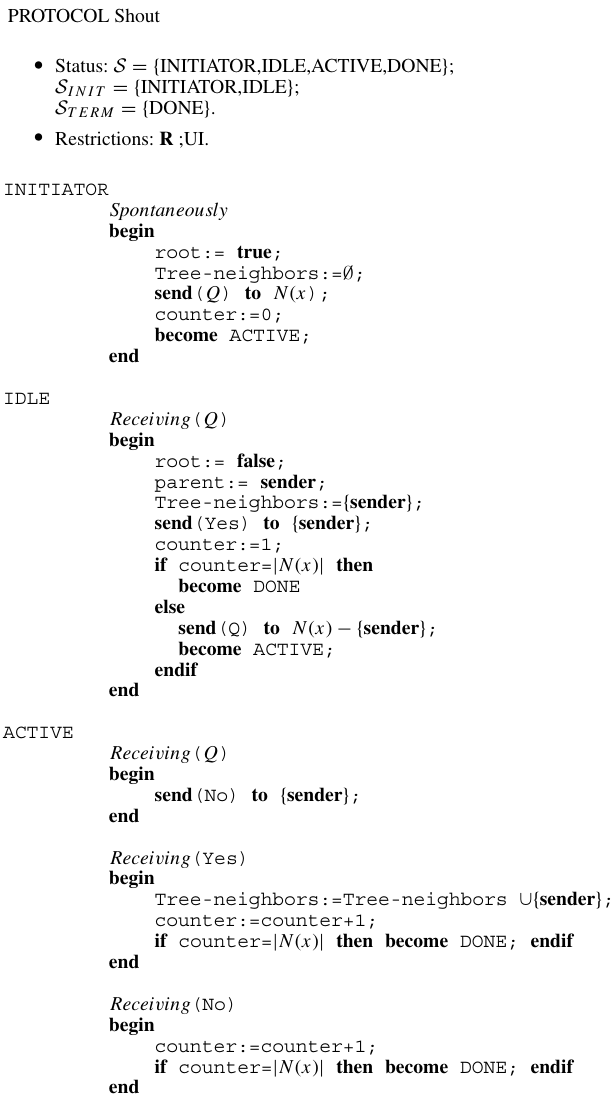
\includegraphics[scale=0.48]{img/shout.png}
				\caption{Algoritmo protocollo shout}
			\end{figure}
		Osservando la struttura dell'algoritmo è chiaro che risulta dalla composizione dei protocolli \textbf{flooding + reply}.
		\subsubsection{Correttezza}
			Sappiamo che flooding è corretto e dunque sappiamo che ogni entità riceverà Q e che per costruzione risponderà \textit{yes} o \textit{no} ad ogni Q che riceve.\\ 
			\textbf{ Per provare la correttezza dobbiamo provare che la sotto-rete $G^{1}$ definita da tutti gli alberi di vicini, è uno spanning tree di $G$.}\\
			Sappiamo che:
			\begin{itemize}
				\item Se $x$ è un tree-neighbor di $y$ allora $y$ è un tree-neighbor di $x$;
				\item Se $x$ invia \textit{yes}	ad $y$, allora $x$ è un tree-neighbor di $y$ ed è connesso all'iniziatore da una catena di \textbf{yes};
				\item Ogni $x$ (a parte l'iniziatore) risponde \textit{yes} solo una volta (quando diventa \textbf{active} risponde no ad ogni richiesta).
			\end{itemize}
			\textbf{Poichè ogni entità $x \neq y$ invia un solo \textit{yes} allora $G^{1}$ contiene tutte le entità di G, è connesso e non contiene cicli e dunque è uno spanning tree di G.}\\
			Importante ricordare che Shout termina per \textbf{terminazione locale} ovvero che ogni entità conosce quando la propria esecuzione è terminata (quando entra nello stato \textbf{done}). Nemmeno l'iniziatore è a conoscenza della \textbf{terminazione globale} (situazione molto comune in un algoritmo distribuito).
		\subsubsection{Costo computazionale}
			Dal momento che shout è definito come flood + reply studiarne la complessità risulta essere molto semplice: 
			$$Message(SHOUT) = 2Message(FLOOD) = 4m-2n+2 $$
			Dal momento che $O(m)$ è un \textbf{lower bound} diciamo che shout è \textbf{asintoticamente ottimo.}
			Nello specifico:
			\begin{figure}[h!]
				\centering
				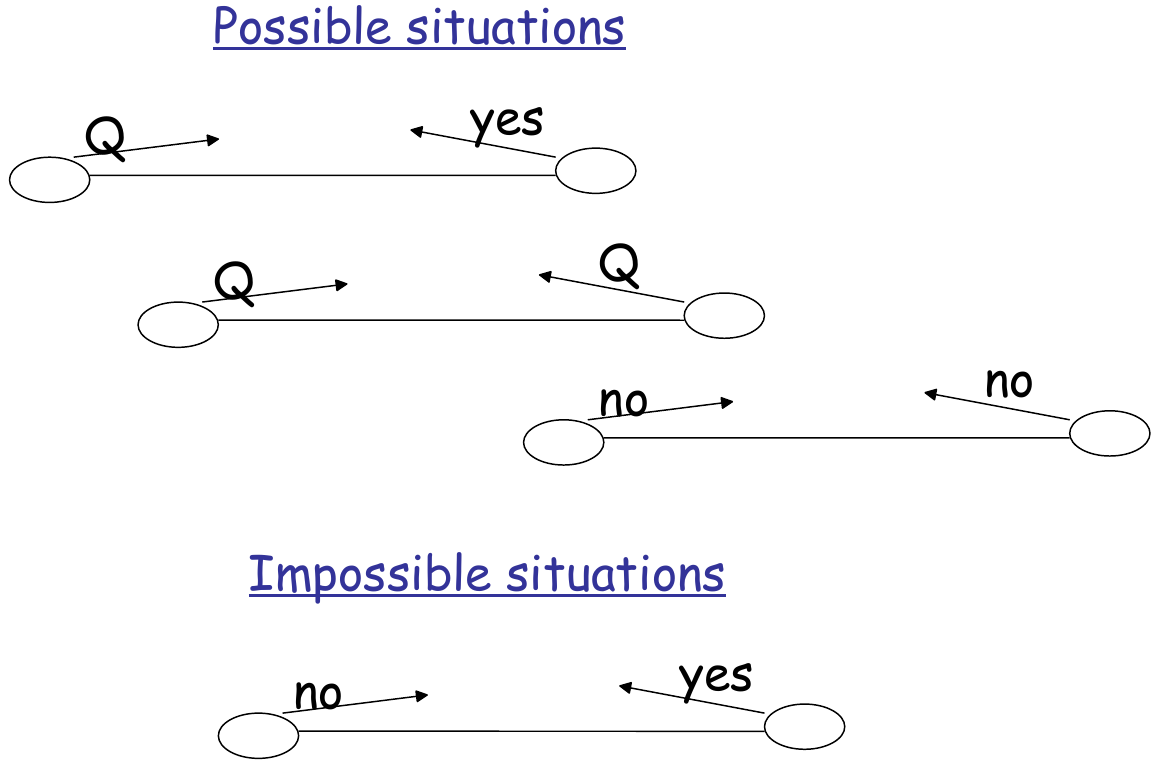
\includegraphics[scale=0.25]{img/shout1.png}
				\caption{Shout: possibili situazioni}
			\end{figure}
			\begin{figure}[h!]
				\centering
				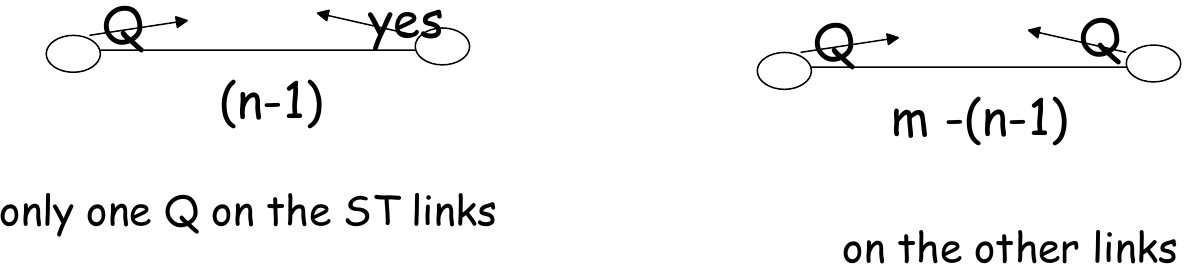
\includegraphics[scale=0.25]{img/shoutmess.png}
				\caption{Totale dei messaggi Q (sei mio vicino?)}
			\end{figure}
			\begin{figure}[h!]
				\centering
				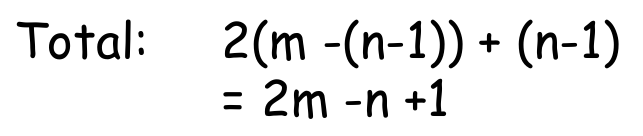
\includegraphics[scale=0.25]{img/shoutmess1.png}
				\caption{Totale dei messaggi Q: formula}
			\end{figure}
			\begin{figure}[h!]
				\centering
				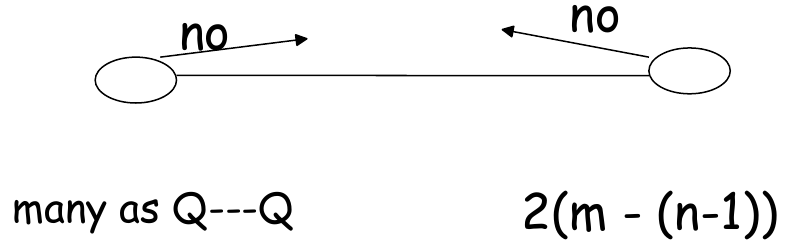
\includegraphics[scale=0.250]{img/numbno.png}
				\caption{Totale dei messaggi no}
			\end{figure}
			\begin{figure}[h!]
				\centering
				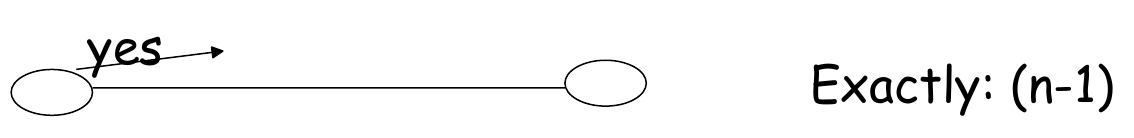
\includegraphics[scale=0.25]{img/numbyess.png}
				\caption{Totale dei messaggi yess}
			\end{figure}
			\begin{figure}[h!]
				\centering
				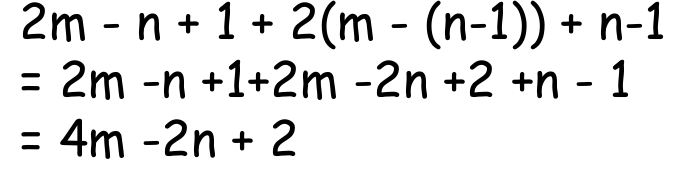
\includegraphics[scale=0.25]{img/totmess.png}
				\caption{Totale dei messaggi scambiati}
			\end{figure}
		
			\newpage
		\subsubsection{Possibili migliorie}
			\textit{Possiamo modificare l'algoritmo in modo tale da eliminare i messaggi \textbf{no}}. Ricordiamo che i delay di consegna dei messaggi sono assunti finiti ma sono per definizione impredicibili. Non possiamo dunque fare a meno dei messaggi di no in quanto non possiamo semplicemente attendere lo scadere  dell'upper-bound di consegna dei messaggi per capire se un'entità risponderà $yes$ o meno. la in quanto sono utilizzati per la terminazione local Per farlo si interpretano i messaggi Q ricevuti come dei no (vedi figura).  La complessità si riduce a:
			$$Messages(SHOUT) = 2si o menom$$
			\begin{figure}[h!]
				\centering
				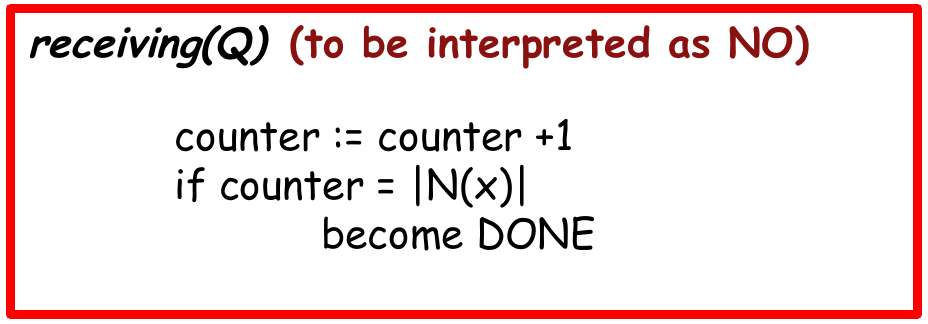
\includegraphics[scale=0.25]{img/shoutmod.png}
				\caption{Shout senza messaggi no}
			\end{figure}
			Un'altra possibile miglioria è implementata con lo scopo di ottenere \textbf{terminazione globale} per l'algoritmo. Si introducono degli \textbf{ACK} che permettono di notificare alla root quando terminare globalmente l'algoritmo. L'idea è quella di introdurre una procedura \textbf{CHECK} che permette ad un nodo, alla ricezione di un messaggio e qualora tutti i propri vicini abbiano risposto, di controllare di essere una \textbf{foglia}: in caso affermativo la foglia invia un \textbf{ACK} al proprio parent. Il parent attende di ricevere un ACK dai tutti i figli per inviare un ACK al padre. Una volta che l'ACK giunge alla root, quest'ultima fa partire dei messaggi di \textbf{termination}. In poche parole gli ACK si muovono dalle foglie verso la radice, mentre i messaggi di termination svolgono il percorso contrario.
			\begin{figure}[h!]
				\centering
				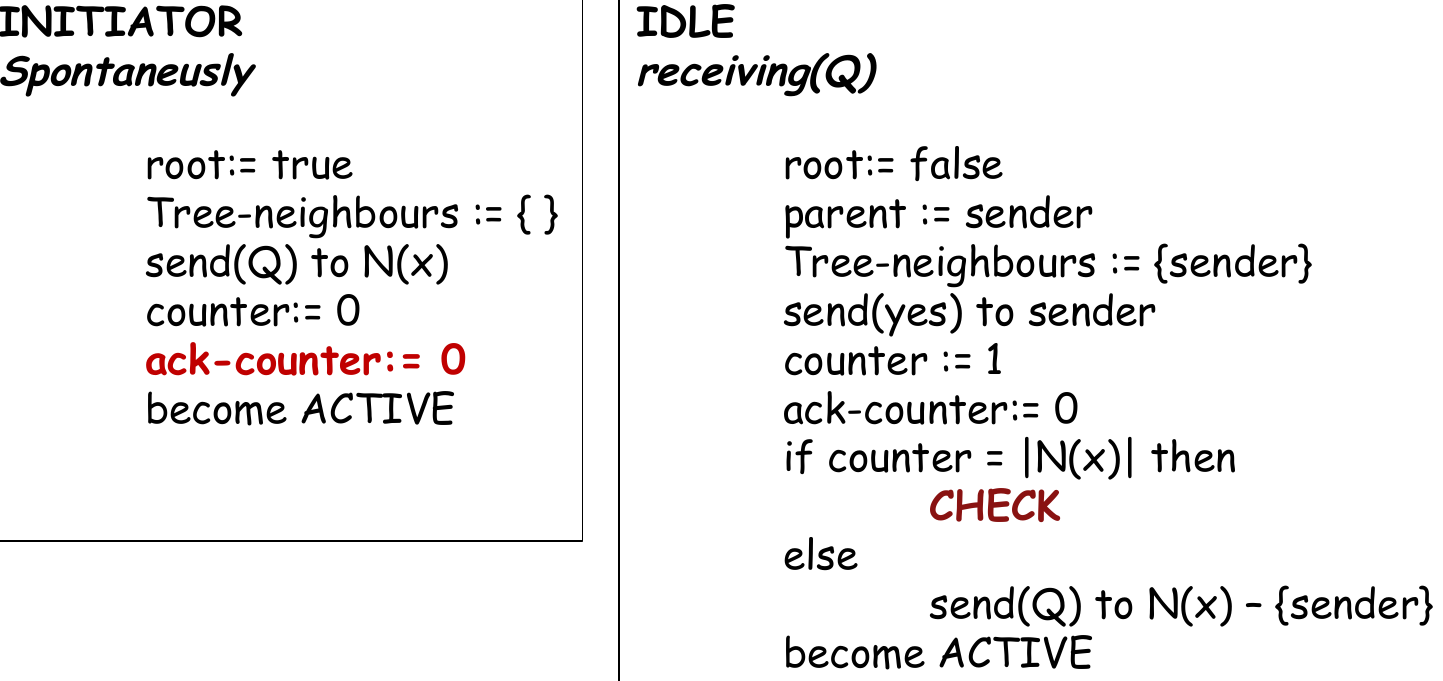
\includegraphics[scale=0.30]{img/shoutterm.png}
				\caption{Algoritmo Shout con global termination 1}
			\end{figure}
			\begin{figure}[h!]
				\centering
				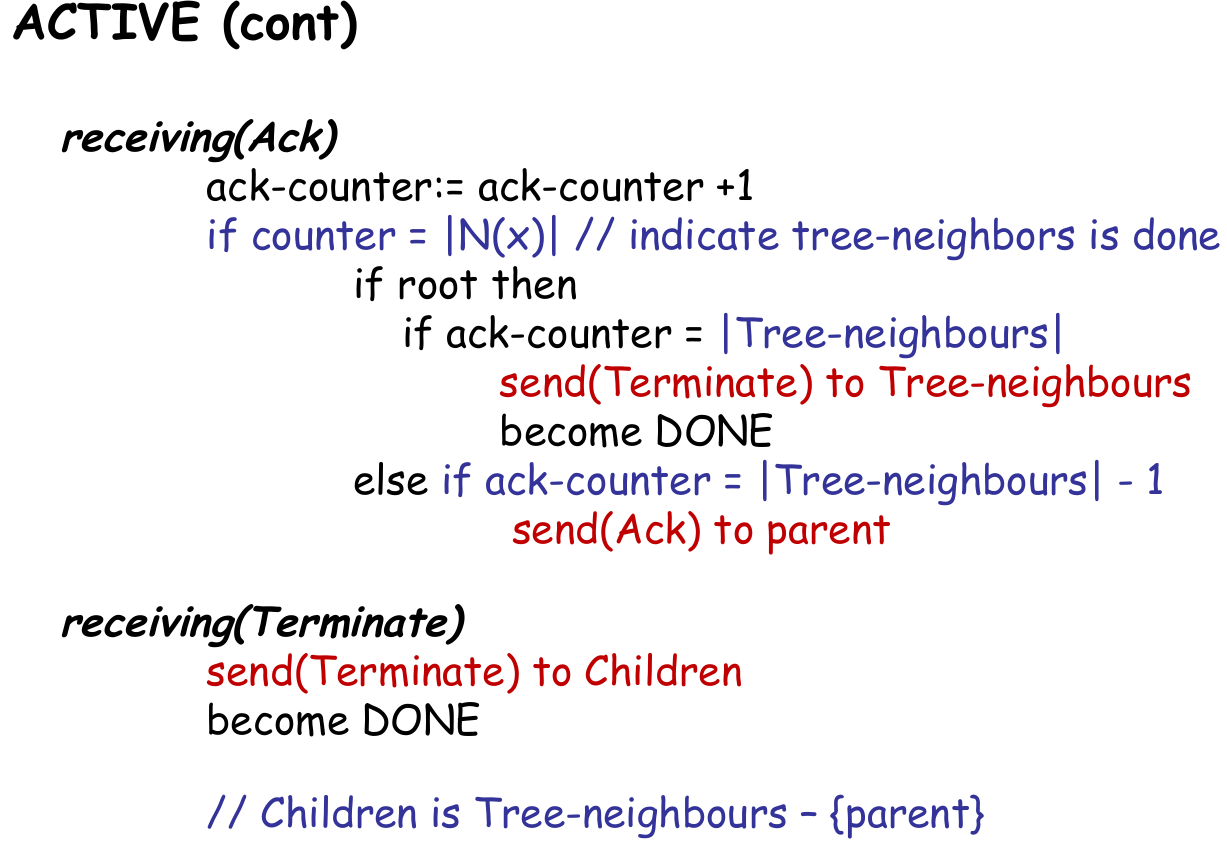
\includegraphics[scale=0.30]{img/shoutterm2.png}
				\caption{Algoritmo Shout con global termination 2}
			\end{figure}
			\begin{figure}[h!]
				\centering
				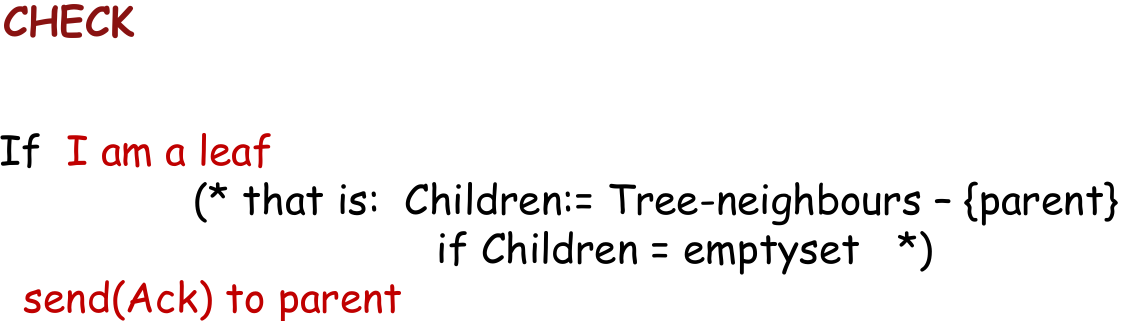
\includegraphics[scale=0.30]{img/shoutterm3.png}
				\caption{Algoritmo Shout con global termination}
			\end{figure}
		\newpage
		
		\subsubsection{Iniziatore mutliplo}
			Abbiamo implementato l'algoritmo \textit{shout} assumendo l'esistenza di un \textbf{iniziatore unico}. Tuttavia questa è un'assunzione molto forte da considerare per un sistema distribuito. In figura si mostra cosa accade nel caso di multipli iniziatori: presi i nodi $x$, $y$, $z$ connessi l'uno con l'altro, con $x$ e $y$ iniziatori, si vede facilmente che se il messaggio Q inviato da $x$ arriva prima a $z$ allora i link $(x,y)$ e $(y,z)$ non saranno presenti nello spanning tree. L'algoritmo di fatto costruisce una \textbf{spanning forest} non connessa.
			\begin{figure}[h!]
				\centering
				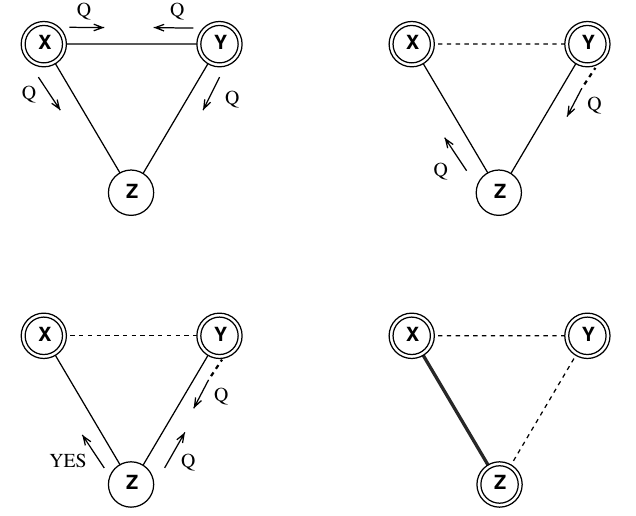
\includegraphics[scale=0.35]{img/multip.png}
				\caption{Iniziatori multipli in Shout}
			\end{figure}
			Questo risultato particolare è avvallato dal \textbf{risultato di impossibilità}:\\
			\textbf{Teorema:} \textit{il problema della costruzione di un spanning tree è deterministicamente impossibile assumendo R.} \\
			Ciò significa che non esiste un protocollo deterministico che termina sempre in tempo finito.
			La prova viene data per assurdo: l'idea è che le entità hanno lo stesso codice e perciò, iniziando simultaneamente nello stesso stato, riceveranno gli stessi messaggi e svolgeranno le stesse computazioni, trovandosi sempre negli stessi stati (tutte le entità sono iniziatori). Il protocollo per essere corretto deve terminare in questa configurazione: x ha la label 2 nella lista, y ha la label 1, mentre z le ha tutte e due. L'assurdo si rileva nel fatto che le entità avrebbero valori distinti anche se gli stati e le computazioni svolte risultano le stesse. \\
			\begin{figure}[h!]
				\centering
				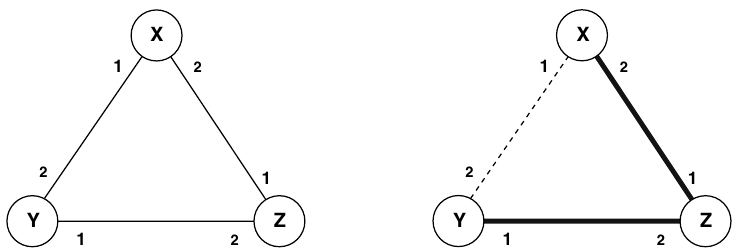
\includegraphics[scale=0.35]{img/imposprove.png}
				\caption{Prova risultato impossibilità}
			\end{figure}
			Se vogliamo costruire uno spanning tree in un contesto distribuito abbiamo dunque bisogno di un algoritmo che esegue la \textbf{leader election}.
			
		\subsubsection{SPT: Depth First Search}
			Sappiamo che una visita in profondità di un grafo restituisce uno spanning tree di tale grafo.
			L'idea è quella di utilizzare un token per identificare il nodo corrente: 
			\begin{itemize}
				\item Quando un nodo viene visitato per la prima volta, tiene traccia di chi è il mittente ed inoltra il token ad uno dei suoi vicini non ancora visitati.
				\item Quando un vicino riceve il token, se è già stato visitato marca l'arco come \textbf{back-edge} e restituisce il token, altrimenti inoltra sequenzialmente il token a tutti i suoi vicini sequenzialmente.
				\item Se non ci sono più vicini non visitati ritorna il token (\textbf{reply}) al nodo dal quale per primo ha ricevuto il token.
				\item Una volta ricevuto un reply, inoltra il token ad un altro vicino non visitato. 
			\end{itemize}
			\begin{figure}[h!]
				\centering
				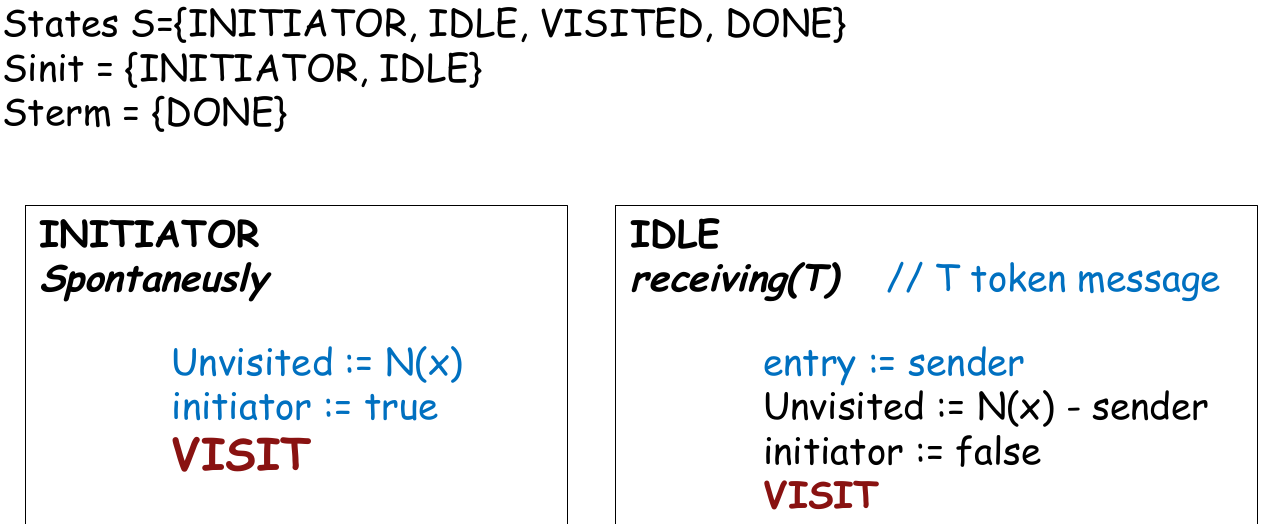
\includegraphics[scale=0.3]{img/dfs.png}
				\caption{Algoritmo DFS 1}
			\end{figure}
			\begin{figure}[h!]
				\centering
				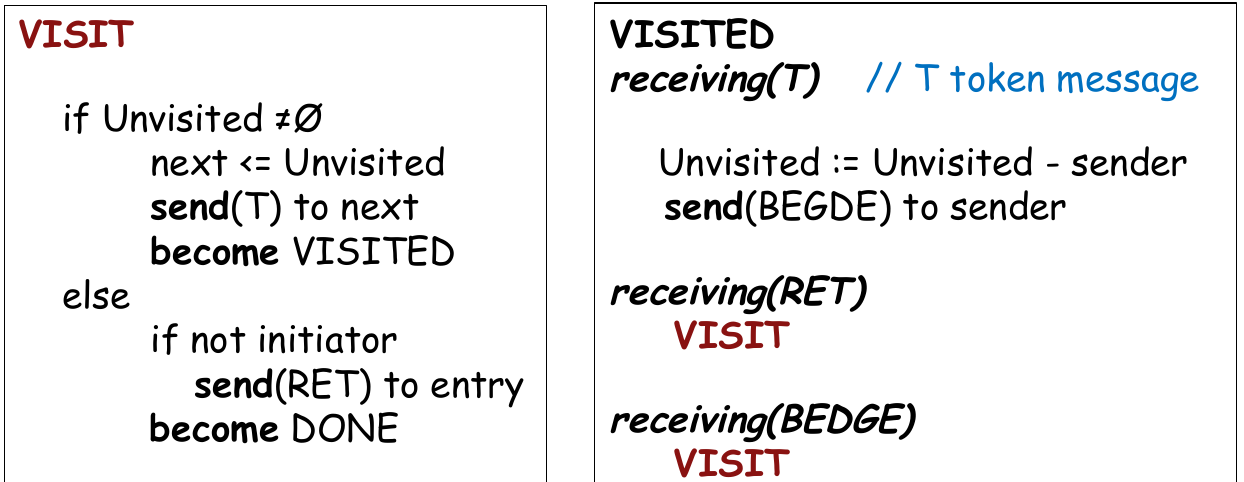
\includegraphics[scale=0.3]{img/dfs2.png}
				\caption{Algoritmo DFS 2}
			\end{figure}
		
			FARE IMMAGINE CON SLIDE DA 30 a 41\\
			
			Per quanto riguarda la \textbf{complessità in messaggi} abbiamo che i messaggi per link sono 2 ( il destinatario del token risponde return se visitato la prima volta o back se già visitato). Dunque:
			$$2m = O(m) $$ con $$O(m) = lower bound $$
			Allo stesso modo la \textbf{complessità in tempo} risulta essere: 
			$$2m = O(m) $$ 	con $$O(n) = lower bound $$
		
		\subsubsection{DF: migliorie}
			Una prima idea è quella di eliminare i messaggi \textbf{back} che costituiscono la maggioranza del totale dei messaggi inviati. Per farlo utilizziamo \textbf{notification} e i messaggi di \textbf{ACK}. 
			\begin{itemize}
				\item L'idea è che il nodo corrente informa i suoi vicini di essere stato visitato.
				\item I vicini rispondono con messaggi di ACK. 
				\item Il mittente dunque segna tutti gli archi dal quale riceve risposta come back-edge.
				\item Sceglie un vicino da visitare e marca quel link come appartenente allo spanning tree. 
			\end{itemize}
			
			INSERIRE IMMAGINI SLIDE 44-48\\
			
			Per quanto riguarda la \textbf{complessità in messaggi} abbiamo che ogni entità riceve un \textbf{token} ed invia un \textbf{return} $$2(n-1)$$
			Inoltre ogni entità invia 1 \textbf{visited} a tutti i vicini tranne al mittente (lo stesso vale per i messaggi di ACK).
			$$\sum|N(s)|+\sum_{x\neq s}(|N(x)|-1) $$
			Il totale è dunque $4m $
			Per quanto riguarda la \textbf{complessità in tempo} abbiamo che i l'invio dei Token e il Return sono inviati sequenzialmente con complessità $2(n-1)$ mentre l'invio degli ack e dei messaggi visited è svolto in parallelo con complessità $2n$. Il totale risulta $$4n-2	$$
			
			FINIRE DF++\\
			
\section{Computazione negli alberi}		
	In questa sezione è analizzato il contesto delle computazioni distribuite in una topologia in forma di \textbf{albero}. Anche in questo caso valgono le restrizioni standard definite da \textbf{R}, in aggiunta ogni nodo sa se è una \textbf{foglia} o un \textbf{nodo interno} (se ha un solo vicino o più di uno).
	
	\subsection{Saturation}  
		La \textbf{Saturazione} è una tecnica base che può essere utilizzata come strumento di partenza per eseguire computazioni in un sistema distribuito. Il protocollo si declina in 3 parti: \textbf{Attivazione}, \textbf{Saturazione}, \textbf{Risoluzione}.
		La fase di risoluzione dipenderà dall'applicazione specifica del protocollo (definisce cosa facciamo con i messaggi di saturation ricevuti) anche se solitamente viene utilizzata come fase di notifica per tutte le entità (con lo scopo di ottenere \textit{local termination}). Un protocollo "troncato" come questo è chiamato \textbf{plug-in} (un protocollo nel quale non tutte le entità entrano in stato terminale). Per far si che diventi un protocollo è necessario definire ulteriori azioni da svolgere. \textit{\textbf{Il protocollo può essere avviato da un qualsiasi numero di initiator.}} Vediamo le fasi in dettaglio:
		\begin{enumerate}
			\item \textbf{Attivazione}: questa fase è un semplice \textbf{\textit{wake-up}}. Ogni initiator invia un messaggio di wake-up a tutti i suoi vicini e diventa \textit{active}. Ogni non initiator che riceve il messaggio diviene active a sua volta e inoltra il messaggio ai suoi vicini (escluso il mittente del messaggio)). I nodi già attivi ignorano altri messaggi di wake up. In \textbf{tempo finito} tutti i nodi divengono attivi, incluse le foglie (per le assunzione di \textbf{total reliability} e l'assioma di \textbf{finite comunication delay})
			\item \textbf{Saturazione}: questa fase è inizializzata dalle foglie che inviano il messaggio \textbf{M} di saturazione al loro unico vicino (il parent), entrando così nello stato di \textbf{\textit{processing}}. Invece, ogni nodo intermedio attende di ricevere un messaggio di saturation da tutti i suoi vicini meno uno. All'ultimo vicino rimasto ed identificato dunque come il parent, il nodo intermedio invia un messaggio di saturation (entrando nello stato \textit{processing}). Se un nodo nello stato di processing riceve un messaggio dal parente allora entra nello stato \textit{\textbf{saturated}}.
			\item \textbf{Risoluzione}: dipende dall'applicazione.	
		\end{enumerate}	
		
		\begin{figure}[h!]
			\centering
			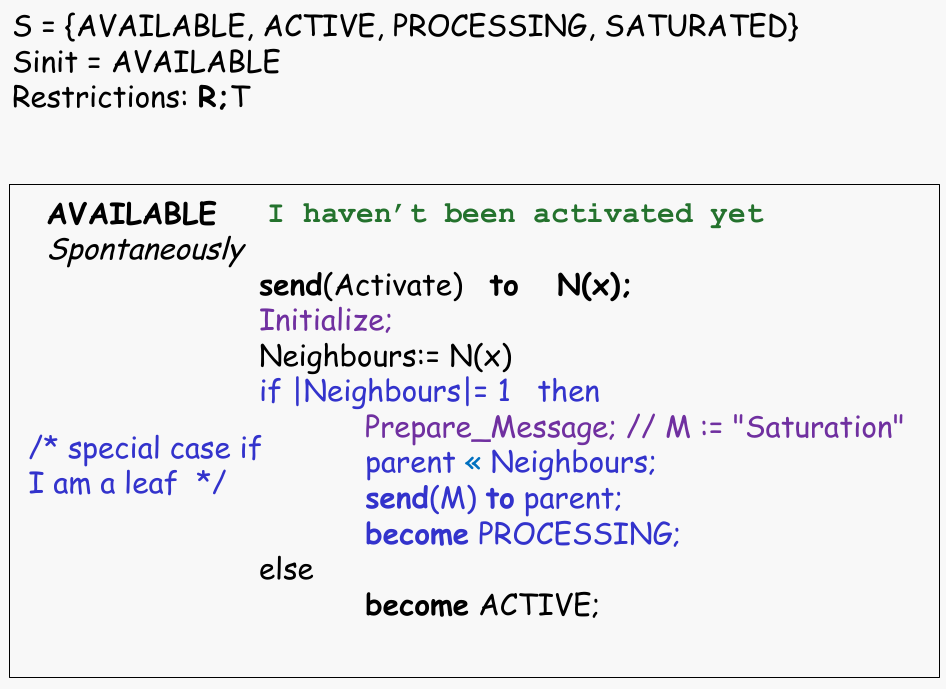
\includegraphics[scale=0.33]{img/sat1.png}
			\caption{Algoritmo Saturazione 1}
		\end{figure}
		\begin{figure}[h!]
			\centering
			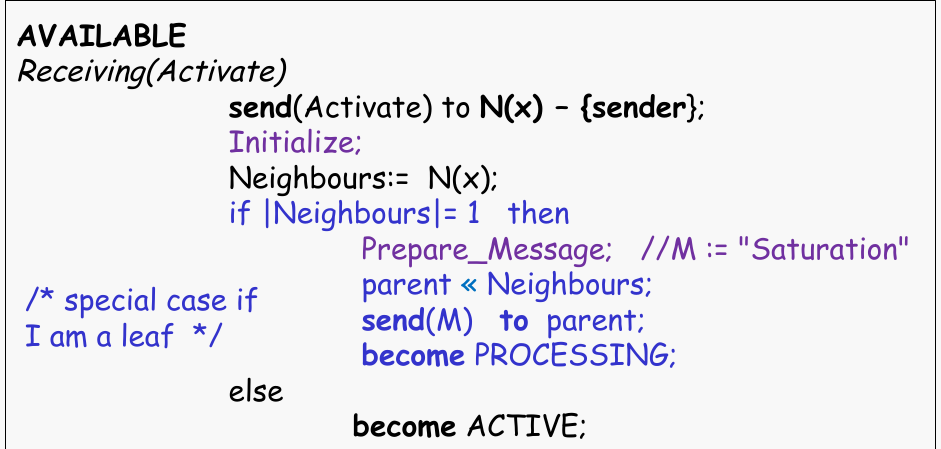
\includegraphics[scale=0.3]{img/sat2.png}
			\caption{Algoritmo Saturazione 2}
		\end{figure}
		\begin{figure}[h!]
			\centering
			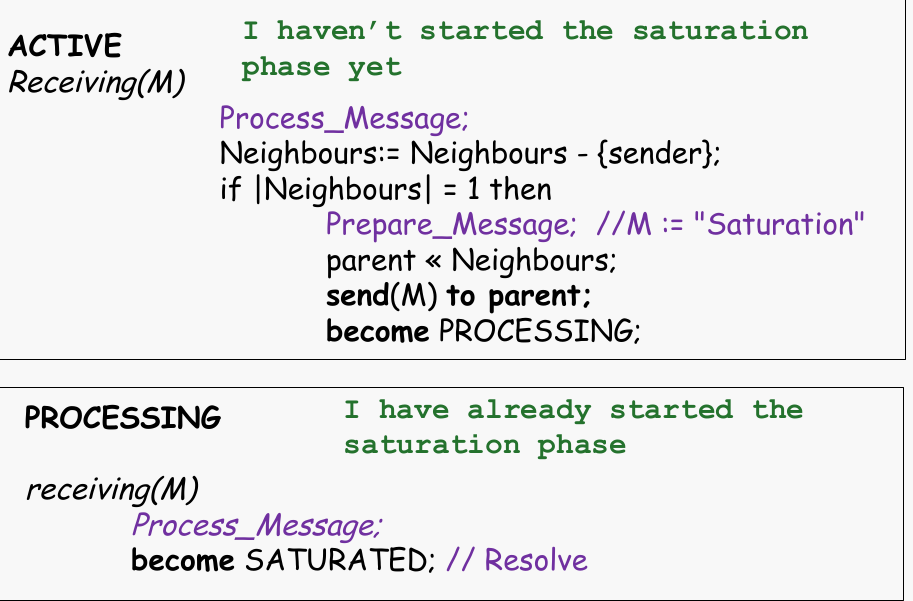
\includegraphics[scale=0.3]{img/sat3.png}
			\caption{Algoritmo Saturazione 3}
		\end{figure}
		
		\subsubsection{Prova di correttezza}
			\textbf{Lemma}: \textit{Esattamente due nodi in stato di processing diventeranno saturati, inoltre questi nodi sono vicini ma anche l'uno il parent dell'altro}\\
			
			\textbf{Prova:} dzal codice sappiamo che un nodo invia il messaggio M solo al suo parente e diviene saturato solo se riceve un messaggio M dal parent. Scegliendo arbitrariamente un nodo della rete $x_{i}$, se attraversiamo gli up-edges (archi che collegano $x_{i}$ al proprio parent) prima o poi troviamo un nodo saturato $s_1$ (questo perchè non ci sono loop nel grafo). Il nodo $s_1$ è diventato saturato perchè ha ricevuto un messaggio da un nodo $s_2$ mentre era nello stato di processing (dunque ha già ricevuto M da un altro nodo quando era active). Dal punto di vista di $s_2$ questo significa che egli è nello stato processing e che considera $s_1$ il suo parent. Dunque, quando $s_2$ riceve un messaggio da $s_1$ questo diventa saturato a sua volta (i due nodi sono l'uno il parent dell'altro). Considerando il caso in cui i nodi saturati sono più di due allora significherebbe che esistono due nodi x,y  saturati per i quali $d(x,y)\leq 2$. Tuttavia se consideriamo un nodo z tra i due nodi x,y vediamo che z non può inviare il messaggio M ad entrambi i nodi e dunque uno dei nodi non può essere saturato. \\
			
			\textbf{Importante}: è impredicibile quale coppia di nodi divenga saturata, questo per via dei delay di consegna dei messaggi ( ovviamente incide anche la scelta degli iniziatori).
			\begin{figure}[h!]
				\centering
				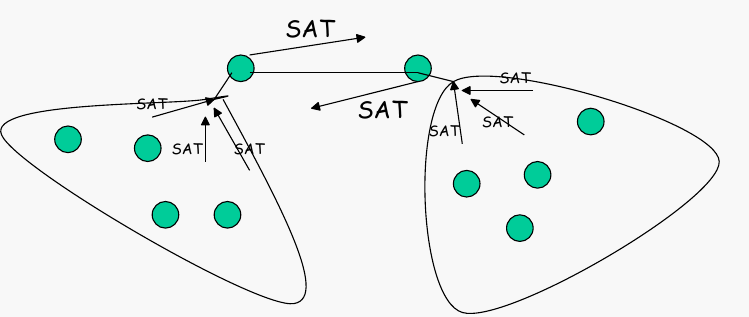
\includegraphics[scale=0.3]{img/satprov.png}
				\caption{Algoritmo Saturazione: prova}
			\end{figure}
		
		\subsubsection{Complessità}
			\begin{figure}[h!]
				\centering
				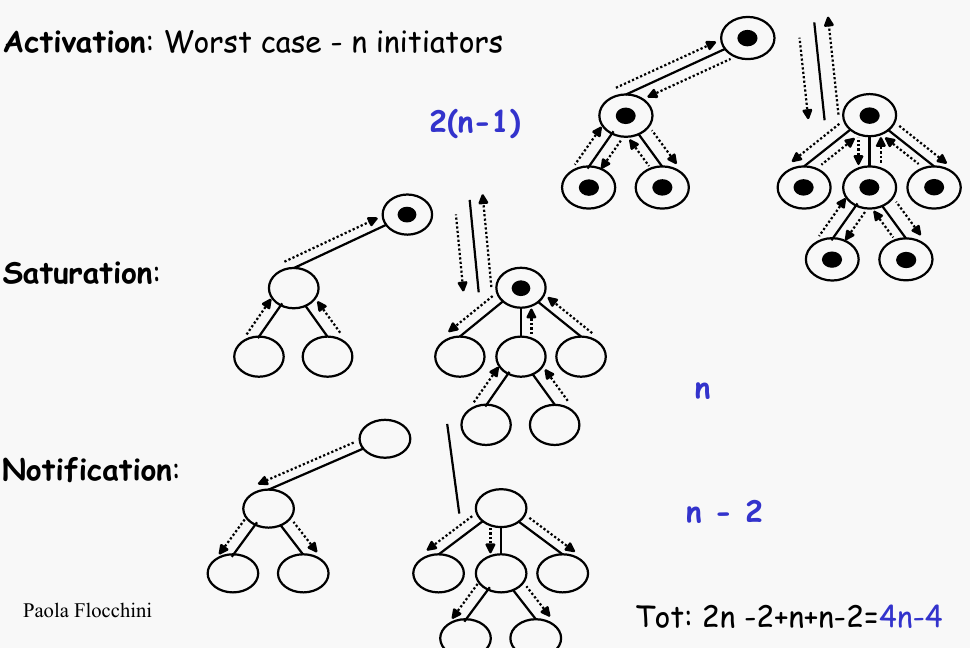
\includegraphics[scale=0.3]{img/satmess.png}
				\caption{Algoritmo Saturazione: complessità caso peggiore}
			\end{figure}
			\begin{figure}[h!]
				\centering
				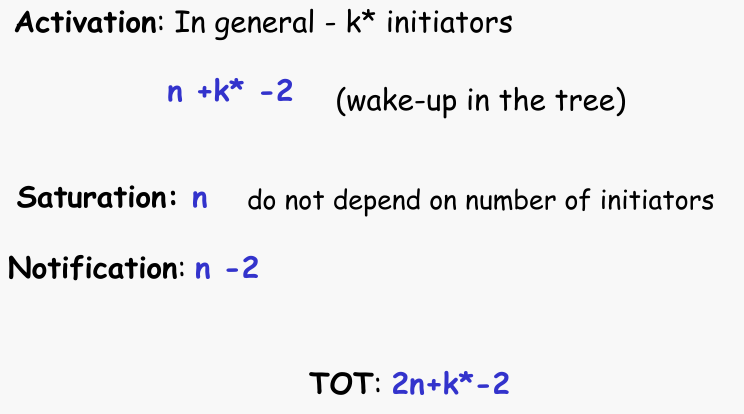
\includegraphics[scale=0.3]{img/satmess2.png}
				\caption{Algoritmo Saturazione: complessità caso generale con n iniziatori}
			\end{figure}
		
		\subsubsection{Ricerca del minimo con saturazione}
			In questa sezione vediamo come si può implementare la fase di risoluzione del protocollo per la ricerca del minimo. In questa configurazione ogni nodo possiede un valore $v(x)$, al termine dell'algoritmo ogni nodo è consapevole di possedere il valore minimo ed entra nello stato appropriato (\textit{minimum} o \textit{large}). Più entità possono avere il valore minimo.\\
			Il problema può essere risolto, nel caso di un rooted tree (esiste un nodo speciale che è la radice e abbiamo orientamento degli archi) eseguendo \textbf{convergecast}: a partire dalle foglie i nodi determinano il valore minimo e lo inviano verso la radice. Il minimo è dunque individuato dalla radice che si occupa di comunicarlo in broadcast agli altri nodi. \textbf{\textit{Assumere l'esitenza di una radice è un'assunzione molto forte:  equivale ad assumere l'esistenza di un leader all'interno della topologia.}} \\
			Per questo motivo usiamo \textbf{saturation} per risolvere il problema senza bisogno di queste informazioni. L'unica modifica effettuata riguarda la fase di processing:
			\begin{figure}[h!]
				\centering
				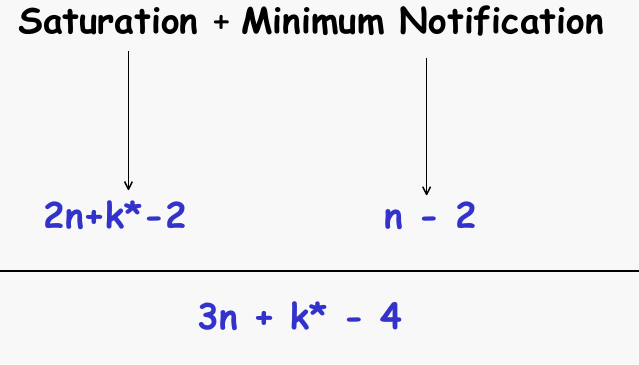
\includegraphics[scale=0.3]{img/mincomp.png}
				\caption{Ricerca minimo con Saturazione: complessità}
			\end{figure}
		
		\subsubsection{Computazione distribuita di funzioni}
			Il problema vede la computazione di una funzione all'interno di un sistema nel quale i suoi argomenti sono distribuiti nei nodi della topologia. \\
			Assumiamo la funzione \textit{f} essere \textit{associativa } e \textit{commutativa}. Questo tipo di funzioni, assieme ai suoi parametri, sono dette \textbf{Semigruppi commutativi}. 
			\begin{figure}[h!]
				\centering
				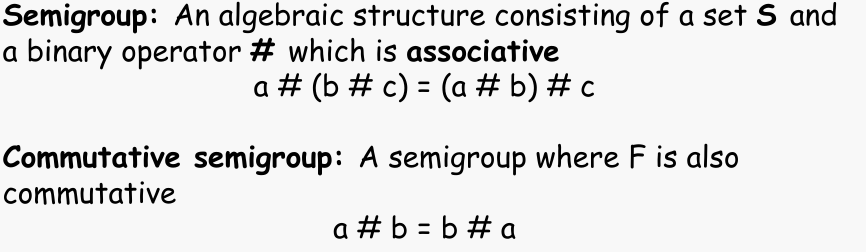
\includegraphics[scale=0.3]{img/semigrup.png}
				\caption{Semigruppi commutativi}
			\end{figure}
			\begin{figure}[h!]
				\centering
				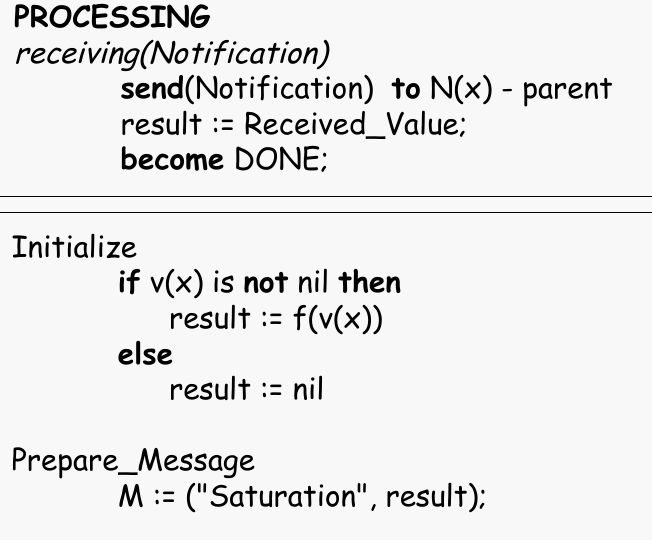
\includegraphics[scale=0.3]{img/distfun.png}
				\caption{Algoritmo computazione distribuita di funzioni 1}
			\end{figure}	
			\begin{figure}[h!]
				\centering
				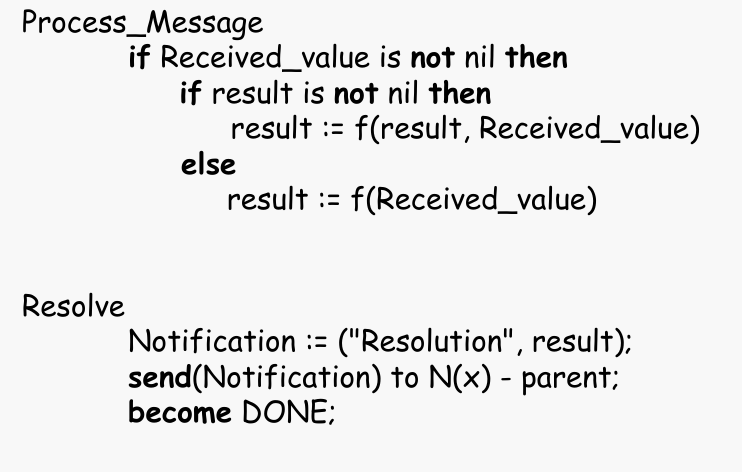
\includegraphics[scale=0.3]{img/distfun1.png}
				\caption{Algoritmo computazione distribuita di funzioni 2}
			\end{figure}
			\begin{figure}[h!]
				\centering
				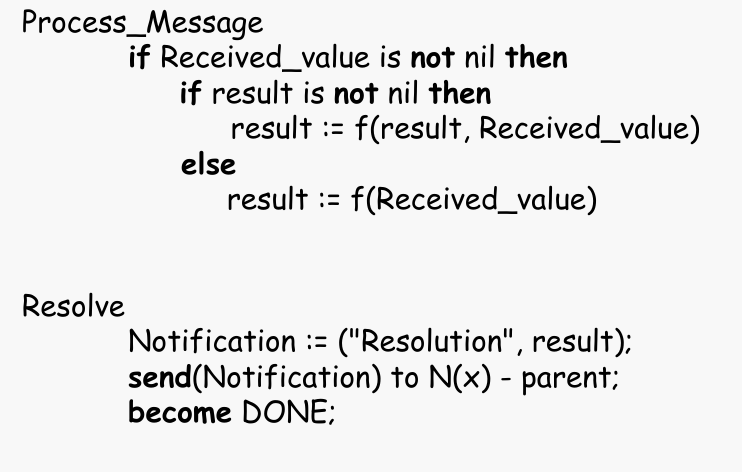
\includegraphics[scale=0.3]{img/distfun1.png}
				\caption{Computazione distribuita di funzioni: complessità}
			\end{figure}
			
		
		
				
			
				   
			
		
			
			
			
			
		
		
			 
			
					 
			 
	
		
		
		
			
		


	

	
	
	
	
		
		
		
	
		
		 
		
		
		  
			
			
			 
			 
	
		
		
		    
			
			 
			
			
			
		
		
			 
		
			 
			
			
			 
			
		
		
		
				
			
				
				
			
		
		
		
		
		
		
		
		
		
		
		
		
		
		
		
		
		
		
		
		
		
		
		
		
		
		
		
		

\end{document}